%%%%%%%%%%%%%%%%%%%%%%%%%%%%%%%%%%%%%%%%%%%%%%%%%%%%%%%%%%%%%%%%%%%%%%%%%%%%%%%%%
%% Paper B -- Target: Environment Systems and Decisions (Springer), Q2
%% Carbon-aware storage-architecture selection for image-based time-series in
%% green IoT (three-way: MongoDB vs PostgreSQL-BYTEA vs PostgreSQL+MinIO).
%%
%% This manuscript consolidates two conference drafts (Postgre-vs-MongoDB and
%% Postgre-vs-Postgre+MinIO) into ONE three-way study and is now backed by a unified,
%% object-oriented benchmark harness that measures per-resolution carbon
%% DIRECTLY (one CodeCarbon tracker per engine x dimension x resolution) over a
%% single 360p->6K sweep with a common retrieval workload across all engines.
%% Data: ../data/ (collage, i9), ../data_collage_i7/, ../data_frames_*/ (real case)
%% Figures: ../figures/   Harness: ../code/   Recorder: ../code_realcase/
%%%%%%%%%%%%%%%%%%%%%%%%%%%%%%%%%%%%%%%%%%%%%%%%%%%%%%%%%%%%%%%%%%%%%%%%%%%%%%%%%

\documentclass[pdflatex,sn-basic]{sn-jnl}% Basic Springer Nature reference style (name-year). Add ",Numbered" if ESD requires numbered citations.

\usepackage{graphicx}%
\usepackage{multirow}%
\usepackage{amsmath,amssymb,amsfonts}%
\usepackage{booktabs}%
\usepackage{xcolor}
\usepackage{array}
\newcolumntype{L}[1]{>{\raggedright\arraybackslash}p{#1}}%
\usepackage{textcomp}%
\usepackage{manyfoot}% required by sn-jnl (table footnotes / \SetFootnoteHook)
\usepackage{listings}%

\graphicspath{{figures/}{../figures/}}

% A small MongoDB-shell (JavaScript) language, since the listings package
% ships SQL but not JavaScript; visual styling is set in \lstset below.
\lstdefinelanguage{MongoJS}{
  morekeywords={db, var, let, const, function, return, true, false, null, new,
    ISODate, BinData, createCollection, createIndex, insertMany, find, sort,
    limit, aggregate, timeseries, timeField, metaField, granularity},
  sensitive=true,
  morecomment=[l]{//},
  morecomment=[s]{/*}{*/},
  morestring=[b]"
}

\lstdefinelanguage{PgSQL}[]{SQL}{
  morekeywords={BIGSERIAL,TIMESTAMPTZ,BYTEA,BIGINT,INTEGER,TEXT},
  morecomment=[l]{--}
}

\lstset{
  basicstyle=\ttfamily\scriptsize,
  keywordstyle=\color{blue}\bfseries,
  commentstyle=\color{gray}\itshape,
  stringstyle=\color{red},
  showstringspaces=false,
  breaklines=true,
  frame=lines,
  numbers=left,
  numberstyle=\tiny\color{gray},
  numbersep=6pt,
  xleftmargin=1.4em,
  framexleftmargin=1.4em,
  backgroundcolor=\color{lightgray!10},
  tabsize=2,
  columns=fullflexible}

% Float placement: with many floats the defaults push them to the
% end of the document. These values let LaTeX place them near their text.
\setcounter{topnumber}{3}
\setcounter{bottomnumber}{2}
\setcounter{totalnumber}{4}
\renewcommand{\topfraction}{0.9}
\renewcommand{\bottomfraction}{0.8}
\renewcommand{\textfraction}{0.07}
\renewcommand{\floatpagefraction}{0.75}

\raggedbottom

\begin{document}

\title[Carbon-aware storage selection for image-based time-series in green IoT]{Carbon Footprint and Carbon-Aware Selection of Document-Oriented, Relational, and Hybrid Object-Relational Storage for Image-Based Time-Series Workloads in Green IoT}

% Author, affiliation, and email details removed for double-anonymous review.
\author*[1]{\fnm{}\sur{[Hidden for Double-blind Review]}}\email{}

\affil*[1]{\orgname{[Hidden for Double-blind Review]}}

\abstract{Smart-building and facility-monitoring deployments increasingly retain high-resolution image streams alongside timestamped metadata in a continuously running data tier, so the choice of storage backend is now a sustainability decision as much as a performance one. This paper measures and compares the carbon footprint of three storage architectures for image-based time-series workloads: the document database MongoDB (image embedded in each record), the relational database PostgreSQL/TimescaleDB (image inline in a binary column), and a hybrid that keeps metadata in PostgreSQL while offloading images to MinIO object storage. Using isolated containers and CodeCarbon with the processor's hardware energy counters, we benchmark resolutions from 360p to 6K, measuring carbon directly for every architecture, resolution, and operation under a common workload. The results reveal a payload-dependent \emph{emission crossover with no universal winner}. Under a profile counting one insertion, one bulk retrieval and one latest-frame read equally, MongoDB is greenest at small payloads, up to 1440p under this workload, whereas the PostgreSQL+MinIO hybrid is greenest at 4K and above, roughly halving inline-storage emissions by decoupling the multi-megabyte payload from the database write path. MongoDB and the hybrid are mirror images, with inline PostgreSQL the pivot across the whole range. MongoDB cannot store 6K frames at all under the default bucketing of a native time-series collection: it packs several multi-megabyte images into one document that breaches the hard 16~MiB limit, a ceiling no hardware raises. On a memory-constrained host the practical limit arrives earlier still, at 4K, where its uncompressed working set exceeded available memory and the process was terminated while the other two architectures completed every resolution. We translate the measurements into a carbon-aware decision framework, with the payload-size regime in which each architecture is greenest, and a measurement procedure for locating those boundaries in another installation, and report Software Carbon Intensity, multi-region grid sensitivity, embodied-carbon implications of storage amplification, and a fleet-scale projection. The same ordering is observed against a corpus of real camera frames recorded from an operational deployment on two cameras, and the controlled sweep is repeated in a second computing environment; each experiment varies several factors at once, so what is established is consistency across the tested host and corpus combinations rather than hardware independence. The selection is shown to depend on the operation profile as well as the payload: a continuously capturing deployment, which writes far more often than it reads, selects inline PostgreSQL at a payload where the equal-weight profile selects MongoDB. A controlled comparison isolates a measurement effect that matters for anyone benchmarking such systems: storing one repeated image rather than distinct ones understates MongoDB's ingestion carbon by a factor of $2.4$ to $2.9$ and its storage amplification by $16$ to $25$, because it alone compresses across rows, while the ordering itself is unaffected. The study is deliberately bounded, and its main limitations should be read alongside its conclusions: measurements come from a single-host, single-client controlled baseline rather than a distributed multi-tenant deployment, and cover the storage tier alone, excluding the deployment's capture and face-recognition pipeline; each carbon cell is a single integrated measurement, with run-to-run variability reaching $28\%$ on the smaller host; the annual deployment figures are a scenario projection for that workload rather than a saving measured against the installation as it currently runs; payloads are drawn from a limited photographic corpus at resolutions up to 1080p for the real-frame validation; carbon is measured under one national grid intensity, although the \emph{ranking} is grid-invariant because emissions scale linearly with that factor; and the embodied-carbon and fleet-scale figures are first-order estimates built from published factors rather than site-specific measurements.}

\keywords{carbon footprint, green computing, sustainable IoT, time-series databases, image-based storage, decision support, life-cycle assessment, software carbon intensity, PostgreSQL, MongoDB, MinIO}

\maketitle

%%=====================================================================%%
\section{Introduction}\label{sec:introduction}
%%=====================================================================%%

Smart-building and facility-monitoring systems increasingly combine conventional telemetry with image streams from embedded cameras, smart doorbells, inspection devices, and other Internet-of-Things (IoT) edge devices---the expanding network of internet-connected sensors that observe the physical world~\citep{bajera_iot_smart_buildings,alfuqaha_iot_survey}. These applications retain binary media (the raw image files) together with timestamps, device identifiers, and other descriptive metadata so that operators can inspect the latest frame, replay recent events, or query activity over time~\citep{ceec_tsdb_review,jensen_tsms_survey}. Because the \emph{data tier}---the software layer that stores and serves this information---runs continuously (24 hours a day, on-site or at the network edge), its electricity use contributes directly to the operational carbon footprint of the building or infrastructure~\citep{nerc_tsdb_survey}. Data centres and on-premises information-technology (IT) equipment already account for a globally significant and growing share of electricity demand~\citep{masanet_datacenter_energy,shehabi_us_datacenter}, so as green-building standards increasingly account for the carbon cost of IT, the choice of storage system is no longer a purely technical decision: it is an environmental and infrastructure-management one~\citep{ieee_ce_definition}.

Organisations typically reuse general-purpose databases for this role rather than adopting specialised systems~\citep{intuz_iot_databases}. A \emph{database} here is the software that stores, indexes, and retrieves data; three database architectures dominate practice, and they differ chiefly in how they handle the bulky image payload (the data carried in each record). First, \emph{MongoDB}~\citep{mongodb_official} is a \emph{document-oriented} database---it stores each record as a self-contained, flexible document---and offers native Time-Series Collections, a storage mode tuned for timestamped data. It keeps each image embedded \emph{inside} the document in a compact binary form called BSON (Binary JSON, the binary encoding of the JavaScript Object Notation text format)~\citep{mongodb_bson_spec}, written to disk by its WiredTiger storage engine~\citep{mongodb_wiredtiger_storage} after general-purpose Snappy compression~\citep{google_snappy}. Second, \emph{PostgreSQL}~\citep{postgresql_official} is a \emph{relational} database, organising data as tables of rows and columns; with the TimescaleDB extension~\citep{timescaledb_official} it partitions a table into time-based chunks, and its built-in TOAST facility (The Oversized-Attribute Storage Technique) automatically relocates large values such as images into separate ``out-of-line'' storage~\citep{postgresql_toast_docs}. Third, a widely used \emph{hybrid} pattern keeps only the small, queryable metadata in PostgreSQL and offloads the bulky image to a dedicated \emph{object store}---a system specialised for holding large files as standalone objects---such as MinIO~\citep{minio_official} or the Amazon Simple Storage Service (S3)~\citep{aws_s3_official}. Because these designs move, copy, and compress the image differently, they can consume very different amounts of energy as image resolution---and therefore payload size---grows.

Existing time-series benchmarks (standardised performance tests) target lightweight numeric events~\citep{tsbs,cratedb_ts_benchmark,diva_timescaledb_mongodb_eval} and rarely evaluate multi-megabyte image payloads; even more rarely do they report energy use or carbon-dioxide-equivalent (CO\textsubscript{2}eq) emissions---the standard unit that converts the warming effect of all greenhouse gases into an equivalent mass of carbon dioxide. This leaves a practical gap for image-heavy IoT deployments that must decide which storage architecture minimises both execution time and carbon, and under which operating conditions. The gap matters because a storage system's behaviour changes fundamentally with payload size, so a conclusion drawn at one resolution need not hold at another.

This paper addresses the following research question: \emph{What is the carbon footprint of document-oriented, relational, and hybrid object-relational storage for image-based time-series workloads across increasing camera resolutions, and how should an operator choose among them to minimise emissions in green IoT infrastructure?} To answer it, we benchmark the three architectures across eight image resolutions from 360p to 6K, stored as JPEG files (Joint Photographic Experts Group, the ubiquitous lossy photo-compression standard)~\citep{wallace_jpeg}. Each architecture runs in its own isolated software container managed by Docker~\citep{docker_official}---a tool that packages software with its dependencies for reproducible execution---and we measure electricity use and emissions with CodeCarbon~\citep{codecarbon}, an open-source tool that records energy and estimates the resulting carbon by reading the processor's built-in Running Average Power Limit (RAPL) energy counters~\citep{david_rapl}, which report the actual energy drawn by the central processing unit (CPU) and memory. We analyse insertion throughput (how fast images are stored), retrieval latency (the delay in reading them back), storage amplification (disk space used relative to the raw data), and \emph{directly measured} per-resolution carbon. Unlike earlier conference studies [hidden for double-blind review], every resolution is measured under its own energy tracker (removing the need to estimate), and a single common read workload is applied to all three systems. We frame storage selection as an \emph{environmental-systems decision}---one that weighs operational and embodied carbon against performance and operational complexity for a given deployment's resolution mix and electricity grid---and the contributions are:

\begin{itemize}
  \item A three-way, directly measured carbon-footprint comparison of MongoDB, PostgreSQL-BYTEA (PostgreSQL storing each image inline in a binary column of type \texttt{BYTEA}, PostgreSQL's ``byte array'' type), and PostgreSQL+MinIO under identical image-based time-series workloads from 360p to 6K, quantifying CO\textsubscript{2}eq emissions with hardware energy measurement.
  \item Evidence of a \emph{payload-dependent emission crossover} in which MongoDB and the hybrid are mirror images---MongoDB greenest at standard resolutions, the hybrid greenest at high resolutions, inline PostgreSQL the pivot---together with the finding that MongoDB cannot store 6K frames at all under the default bucketing of a native time-series collection, because that bucketing breaches the hard 16~mebibyte (MiB) limit on a single BSON document.
  \item An environmental analysis that lifts the result beyond a performance benchmark: Software Carbon Intensity (SCI)---a standardised measure of carbon emitted per unit of useful work, defined by the international standard ISO/IEC~21031:2024~\citep{gsf_sci}---together with a multi-region electricity-grid sensitivity analysis (re-evaluating emissions under different regions' grid carbon intensities)~\citep{owid_carbon_intensity}, the \emph{embodied} carbon (manufacturing emissions) implied by storage amplification~\citep{tannu_ssd_embodied,gupta_chasing_carbon}, and a fleet-scale annual projection.
  \item A \emph{carbon-aware decision framework} that maps measured payload size and workload emphasis to the lowest-emission architecture, together with a short calibration procedure for locating its boundaries at another site, intended as decision support for sustainable building-monitoring infrastructure.
\end{itemize}

%%=====================================================================%%
\section{Related Work}\label{sec:related_work}
%%=====================================================================%%

\textbf{Time-series storage.} Time-series databases are designed for data that mostly arrives in timestamped order and is rarely modified afterwards. They sustain this append-oriented ingestion through time-based partitioning, compression, and storage layouts that reduce \emph{write amplification}---the tendency of a database to write substantially more data to disk than the application supplied, here by repeatedly rewriting the tree-structured on-disk indexes (B-trees) that locate records~\citep{dewaal_timeseries_survey,jensen_tsms_survey}. TimescaleDB~\citep{timescaledb_official} extends PostgreSQL with time-based table partitioning while preserving its standard query language, and MongoDB~\citep{mongodb_official} introduced native Time-Series Collections that \emph{bucket} (group) many measurements into compacted documents~\citep{mongodb_timeseries_collections_guide,mongodb_ts_best_practices}.

\textbf{Benchmarks and the binary-payload gap.} Most comparative benchmarks target lightweight scalar data: TSBS~\citep{tsbs} uses small DevOps/telemetry records, CrateDB's benchmark~\citep{cratedb_ts_benchmark} focuses on numeric IoT metrics, and the evaluation by \citet{diva_timescaledb_mongodb_eval} studies numerical sensor workloads. Among the benchmarks reviewed here, none characterise multi-megabyte image payloads, where the internal design of the storage system becomes decisive, and none report energy or emissions (Table~\ref{tab:relwork}); we make no claim about the literature beyond the studies compared in that table. PostgreSQL's TOAST~\citep{postgresql_toast_docs} relocates oversized values out-of-line but keeps them within the database's transactional and retrieval machinery; MongoDB stores binaries inline in BSON documents~\citep{mongodb_bson_spec}, and its alternative for large files---GridFS, which splits a file into smaller chunks~\citep{mongodb_gridfs}---is incompatible with native Time-Series Collections~\citep{mongodb_ts_limitations}. Object stores such as MinIO~\citep{minio_official} instead stream large, unchanging objects directly while the relational system manages only lightweight metadata. The architectural trade-off is therefore not simply ``one system versus two'' but \emph{one transactional path for everything} versus \emph{separating metadata management from binary transport}.

\textbf{Carbon footprint of computing.} \citet{lannelongue_green_algorithms} formalised the Green Algorithms approach to quantifying the carbon footprint of computation, and \citet{strubell_energy_nlp} highlighted the energy cost of large-scale computation; CodeCarbon~\citep{codecarbon} provides a practical implementation that estimates energy and emissions from machine-level measurements and regional grid intensity. Beyond the energy consumed while running (\emph{operational} carbon), a growing literature stresses \emph{embodied} carbon---the emissions from manufacturing the hardware itself---as a first-class concern for sustainable systems~\citep{gupta_chasing_carbon}, with flash storage a notable contributor~\citep{tannu_ssd_embodied}. Facility-level accounting further multiplies computing energy by the Power Usage Effectiveness (PUE), the ratio of a data centre's total energy draw to the energy that actually reaches its computing equipment, which captures cooling and power-delivery overhead~\citep{shehabi_us_datacenter,masanet_datacenter_energy}. The Software Carbon Intensity specification~\citep{gsf_sci} standardises reporting of emissions per unit of useful work. Within database systems, however, little work applies per-operation carbon accounting to binary time-series storage. This study addresses that gap for document-oriented, relational, and hybrid object-relational image storage, and connects it to embodied carbon, PUE, grid intensity, and SCI.

\textbf{Environmental decision analysis for socio-technical systems.} The framework proposed here is a decision-analysis instrument, and it inherits its structure from a line of work in this journal that couples measured evidence to a selection rule. \citet{bajwa_material_selection_mcdm} survey multi-criteria decision making for material selection in construction and identify a recurring weakness we take seriously: criteria are frequently drawn from the literature rather than measured in the deciding organisation's own context, which limits transferability. Our response is to make the decision variable, payload size, directly measurable by the adopter, and to express the rule as a crossover computed from two constants rather than as a fixed recommendation. \citet{kraft_lca_railway_sensitivity} shows, in a life-cycle assessment of lightweight railway vehicles, that sensitivity analysis is what separates a robust design conclusion from an artefact of the assumed parameters; the multi-region grid-intensity analysis in Section~\ref{subsec:grid} plays that role here, and establishes that our ranking is invariant to the parameter that varies most between deployment locations, national grid intensity differing by more than an order of magnitude across the regions evaluated.

Closer to the deployment we study, \citet{adams_smart_home_energy} estimate energy consumption in a smart home from data-driven simulation, treating the building's instrumentation as the object of environmental analysis. Their concern is the energy the building consumes; ours is the energy consumed by the tier that \emph{stores what the instrumentation records}, which their models do not account for and which we show can be reduced by roughly half through a storage decision alone. \citet{singh_iot_self_healing} and \citet{radanliev_iot_edge_risk} address the operational integrity of IoT systems, namely self-healing through log analytics and real-time risk at the edge, and both presuppose a data tier that durably retains device output. We supply the missing environmental cost of that presupposition. Finally, \citet{alessa_demand_response_review} review price-driven energy management and demand response, where load is shifted in time to exploit a varying grid. Our grid-intensity results (Section~\ref{subsec:grid}) show why that lever is weaker here than it first appears: because emissions are energy multiplied by grid intensity, temporal or geographic shifting rescales every architecture equally and cannot change which one to choose. The saving must come from the architecture itself.

\begin{table}[htbp]
\caption{Representative time-series benchmarks versus this work. We are unaware of prior work that benchmarks multi-megabyte image payloads \emph{and} reports energy/CO\textsubscript{2}. The final column states what each study concludes and what changes once payloads are large enough for the storage engine's internal layout to dominate.}\label{tab:relwork}
\footnotesize
\setlength{\tabcolsep}{3pt}
\begin{tabular}{@{}L{0.155\textwidth}L{0.115\textwidth}L{0.065\textwidth}L{0.115\textwidth}L{0.075\textwidth}L{0.315\textwidth}@{}}
\toprule
Study & Payload type & Max payload & Engines & Energy / CO\textsubscript{2}? & What it concludes / what this work changes \\
\midrule
TSBS~\citep{tsbs} & numeric/scalar & $\sim$KB & multiple TSDBs & No & Ranks engines on ingest of small scalar rows, where throughput is dominated by per-row overhead. We show the ranking inverts once the payload, not the row count, governs the write path. \\
CrateDB~\citep{cratedb_ts_benchmark} & numeric IoT metrics & $\sim$KB & CrateDB et al. & No & Optimises for query latency on numeric metrics; storage volume is incidental. We find storage amplification varies by three orders of magnitude across engines and drives both operational and embodied carbon. \\
\citet{diva_timescaledb_mongodb_eval} & numeric sensor & $\sim$KB & Timescale, Mongo & No & Reports MongoDB ingesting faster than TimescaleDB. Our measurements agree at small payloads and reverse as the payload grows, so the ordering is \emph{payload-dependent} rather than a property of the engines. The comparison is qualitative: the workloads are not the same experiment. \\
\textbf{This work} & \textbf{JPEG images} & \textbf{7.1~MB} & \textbf{Postgre, Mongo, PostMin} & \textbf{Yes (RAPL)} & \textbf{Directly measured per-operation carbon, a payload-dependent emission crossover, a measurement procedure that transfers the rule to other installations, and an infeasibility result at 6K.} \\
\botrule
\end{tabular}
\end{table}

%%=====================================================================%%
\section{Methodology}\label{sec:methodology}
%%=====================================================================%%

\subsection{Hardware and software environment}\label{subsec:env}
All experiments execute on a single computer (Table~\ref{tab:env}) running Ubuntu~24.04.4~LTS (Linux 6.8.0) with an 11th-generation Intel Core i9-11900H processor (8~cores / 16~threads, 2.50--4.90~GHz), 30.99~GB of random-access memory (RAM; the computer's fast working memory), and a 1.9~TB Samsung solid-state drive (SSD; flash-based storage) on the high-speed Non-Volatile Memory Express (NVMe) interface. The host is in Indonesia; CodeCarbon uses the corresponding national grid carbon-intensity factor ($\approx$0.676~kilograms of CO\textsubscript{2}eq per kilowatt-hour, kg~CO\textsubscript{2}eq/kWh), i.e.\ the emissions associated with each unit of electricity consumed. Processor and memory energy are measured directly via the Intel RAPL hardware counters. The three architectures share the same host but run one at a time, in isolation, so that energy is attributed to the architecture under test. A single host with one client issuing requests sequentially is a deliberate \emph{controlled baseline}: it removes scheduling, contention, and network-topology confounds so the measured differences are attributable to each architecture's payload handling---the variable under study---and keeps the comparison fully reproducible. Because the emission crossover is driven by payload size, a structural property of each storage design, multi-client and distributed deployments are expected to shift the absolute figures but not the architectural ordering (Section~\ref{sec:discussion}).

\begin{table}[htbp]
\caption{Hardware and software environment (reproducibility).}\label{tab:env}
\small
\begin{tabular}{@{}ll@{}}
\toprule
Component & Version / setting \\
\midrule
CPU & Intel Core i9-11900H, 8C/16T, 2.50--4.90~GHz \\
RAM / SSD & 30.99~GB / 1.9~TB Samsung NVMe$^{\dagger}$ \\
OS & Ubuntu 24.04.4 LTS (Linux 6.8.0) \\
Containers & Docker 29.4.0, Compose v5.1.1 \\
PostgreSQL & 15 + TimescaleDB (\texttt{latest-pg15}) \\
MongoDB & 7.0 (\texttt{--wiredTigerCacheSizeGB 30}) \\
MinIO & \texttt{minio/minio:latest} \\
Runtime & Python 3.14, \texttt{psycopg2} 2.9.11, \texttt{pymongo} 4.17, \\
        & \texttt{minio} 7.2.20, Pillow 12.2.0, CodeCarbon 3.2.7 \\
Energy & Intel RAPL (CPU+RAM), \texttt{tracking\_mode=machine} \\
Grid factor & 0.676~kg~CO\textsubscript{2}eq/kWh (Indonesia) \\
\botrule
\end{tabular}
\footnotetext{$^{\dagger}$The real-frame validation of Section~\ref{subsec:realframes} ran on a \emph{different} computer, with a four-core Core i7-1165G7 and 15.30~GB of memory; see Table~\ref{tab:env2}. The ordering reported here is the same on both, for the payloads each measured.}
\end{table}

\subsection{Workloads and payloads}\label{subsec:workloads}
The benchmark harness generates deterministic JPEG payloads from a single source image---a freely-licensed photograph of Durdle Door, Dorset, UK~\citep{pexels_durdle_door}, resized to 6144$\times$3456---using a collage transform (Pillow), at quality~90. The payload is therefore genuine photographic content, not computer-generated imagery: what is constructed is the composition, which tiles mirrored and flipped copies of the source to fill each resolution, and, decisively for the measurements, the fact that one such image is stored for every row. Eight resolutions are evaluated: 360p ($640{\times}360$, 0.09~MB), 480p ($854{\times}480$, 0.16~MiB), 720p ($1280{\times}720$, 0.36~MB), 1080p ($1920{\times}1080$, 0.80~MB), 1440p ($2560{\times}1440$, 1.40~MB), 4K~UHD ($3840{\times}2160$, 2.99~MB), 5K ($5120{\times}2880$, 5.09~MB), and 6K ($6144{\times}3456$, 7.13~MB). Quality-90 JPEG retains high visual \emph{entropy}---fine, unpredictable detail that resists further compression---which leaves little for the databases' built-in compression to remove and reflects realistic conditions for storing real photographs. For each resolution the harness performs a 100-row warm-up (untimed priming inserts that bring caches to a steady state), then 5 measured insertion runs of 2{,}000 records each, submitted in batches of~50, followed by 5 measured bulk-retrieval runs and 5 measured latest-frame reads (each preceded by warm-ups). Each database is wiped and rebuilt between resolutions, and only the services needed by the architecture under test are running, so that energy is attributed fairly. Because this construction inserts the same image for every row, a second corpus of real, independently captured camera frames is used to verify that the conclusions do not depend on it; the protocol is identical except that each row receives a different photograph (Section~\ref{subsec:realframes}).

\subsection{Schema and operations}\label{subsec:schema}
\textbf{MongoDB (Mongo).} Each frame is one document in a native Time-Series Collection, with the image stored inline as \texttt{BinData} (BSON's binary type) and the metadata in a nested object; WiredTiger applies Snappy compression when writing to disk. Storing the image inline is the only native option here: MongoDB's large-file facility, GridFS, is incompatible with Time-Series Collections~\citep{mongodb_ts_limitations}, so this configuration reflects MongoDB's \emph{supported} design for timestamped media rather than a deliberately weak setup---the inline path is the one a practitioner adopting native time-series storage would actually use.

\textbf{PostgreSQL-BYTEA (Postgre).} Each frame is one row in a TimescaleDB time-partitioned table, with the image held inline in a \texttt{BYTEA} column and relocated out-of-line automatically by TOAST when it is large~\citep{postgresql_toast_docs}.

\textbf{PostgreSQL+MinIO (PostMin).} PostgreSQL stores the metadata plus a short reference key to the image; the image itself is uploaded to MinIO with an HTTP (Hypertext Transfer Protocol, the request/response protocol of the web) PUT request. Reading back first fetches the key from PostgreSQL and then streams the image from MinIO with an HTTP GET request.

All three architectures maintain a combined index on the device identifier and timestamp that accelerates ``latest-frame'' lookups. We measure four operations per architecture and resolution: (i)~insertion throughput and storage amplification; (ii)~\emph{bulk retrieval} (in database terms, full materialisation), which reads back every one of the 2{,}000 images in a time range and transfers its full content---the access pattern behind reviewing or exporting recent footage; (iii)~\emph{latest-frame read} (a single point read), the time to fetch the most recent image---the access pattern behind a live dashboard; and (iv)~driver round-trip overhead, the fixed cost of one minimal client--server exchange. The full schema, the three queries, and a step-by-step technical walk-through for all three architectures are given in Appendix~\ref{app:schemas}.

The two designs encode the \emph{same} logical record but place the image very differently---inline in the database (PostgreSQL \texttt{BYTEA} or MongoDB \texttt{BinData}) versus externalised to an object store (the hybrid)---which is the root of their contrasting energy profiles.

\subsection{Carbon-footprint measurement}\label{subsec:carbon_method}
Every combination of architecture, operation, and resolution runs inside its own CodeCarbon~\citep{codecarbon} energy tracker, so per-resolution energy and emissions are measured \emph{directly}, rather than estimated by spreading one coarse measurement across resolutions as in earlier work [hidden for double-blind review]. CodeCarbon reads processor and memory power via Intel RAPL and converts the total energy to CO\textsubscript{2}eq using the Indonesian grid intensity. Each tracker encloses an operation's \emph{entire} measurement cell, which is broader than the timed work alone: it covers the untimed warm-up, the database reset performed before each repetition, the five repetitions themselves, and the storage-size and row-count queries taken between them. We divide each integrated measurement by the repetition count and report the result as an \emph{amortised per-run cost}: the energy attributable to one repetition together with its share of the setup that repetition required. This is the unit used throughout for Software Carbon Intensity, per-frame, and scaled figures, and it is deliberately inclusive, since an operator provisioning a data tier pays for resets and warm-up as well as for steady-state writes. It is not, however, the energy of an isolated insert batch in a warm database, and it should not be read as one. The setup component is not identical across architectures---each resets its own storage differently, and the hybrid additionally clears an object-store bucket---so a small part of the difference between architectures is attributable to that work rather than to the payload path. Throughput and latency are reported as means over the five runs with their standard deviations as a measure of run-to-run variability (Tables~\ref{tab:write}--\ref{tab:read}). Their measurement boundary differs from the carbon boundary in one respect that should be stated: the insertion timer stops before the transaction is committed, so reported throughput is an application-side, pre-commit figure, whereas the tracker continues through commit and the accounting queries. Throughput and carbon are therefore reported alongside one another but are not used to explain one another; carbon, by contrast, is a single integrated per-operation measurement and so carries no independent run-to-run dispersion---the small timing variability bounds it. Because emissions are simply energy multiplied by the grid intensity, the \emph{ranking} of the architectures depends on energy alone and is therefore the same in every region (Section~\ref{subsec:grid}).

\subsection{Failover and the unstorable cell}\label{subsec:failover}
To keep the measurements reliable and the data complete, each measurement is held in memory and saved only after it completes successfully; a measurement that fails is retried, and after repeated failures it is recorded as \emph{skipped} (with the architecture, resolution, number of attempts, and error) and the sweep continues to the next case. Exactly one case triggered this path: \textbf{MongoDB at 6K} (Section~\ref{subsec:bson}). The benchmark therefore reports a clean three-way comparison from 360p to 5K and a two-way PostgreSQL-versus-hybrid comparison at 6K, with the omission stated explicitly rather than silently mishandled.

%%=====================================================================%%
\section{Results}\label{sec:results}
%%=====================================================================%%

We report insertion throughput and storage amplification (Section~\ref{subsec:insert}), bulk retrieval and latest-frame reads (Section~\ref{subsec:retrieval}), the central per-resolution carbon comparison with its SCI and embodied-carbon implications (Section~\ref{subsec:carbon}), multi-region grid sensitivity (Section~\ref{subsec:grid}), and MongoDB's 16~MiB ceiling (Section~\ref{subsec:bson}). All values are directly measured on identical hardware and CodeCarbon configuration; run-to-run variability is small for the carbon-dominating insertion and bulk-retrieval operations (coefficient of variation $\approx$1.6\% at the median and $<$8\% in the worst case; Tables~\ref{tab:write}--\ref{tab:read}), so differences of a few percent---such as the MongoDB--PostgreSQL near-tie at 4K---sit within measurement noise, whereas the order-of-magnitude crossovers are unambiguous; the per-operation winners are summarised in the decision framework (Section~\ref{sec:framework}).

\subsection{Insertion throughput and storage amplification}\label{subsec:insert}
Insertion (Figure~\ref{fig:insert}, Table~\ref{tab:write}) exhibits a monotone reordering with payload size. At low resolution MongoDB ingests much faster than the alternatives---4{,}194~rows/s at 360p, over $6\times$ PostgreSQL and $56\times$ the hybrid---because each frame compresses to a near-empty bucket (storage amplification $0.001\times$) that WiredTiger writes entirely in cache. That figure is specific to a workload in which every row holds the same image: MongoDB buckets many rows together and compresses across them, so identical rows all but vanish. Section~\ref{subsec:realframes} measures the same quantity on distinct real frames and finds it an order of magnitude higher. PostgreSQL is the middle ingester at low resolution (batched inserts avoid a per-object network call), while PostMin pays the fixed cost of one MinIO PUT per payload and is slowest. As payloads grow the order inverts: MongoDB falls below PostgreSQL between 1440p and 4K and becomes the slowest engine at 4K--5K as WiredTiger serialises multi-megabyte BSON documents through B-tree pages~\citep{wiredtiger_btree_architecture} and compression no longer helps; PostMin, whose throughput is nearly flat, overtakes PostgreSQL at 4K and remains highest through 6K. Storage amplification (Figure~\ref{fig:storage}) explains much of the downstream carbon: Postgre holds a stable $\sim$1.04$\times$ (TOAST out-of-line layout) and PostMin $\sim$1.00$\times$ (raw object size) at all resolutions, whereas MongoDB changes sharply---$0.10\times$ at 1080p (Snappy compresses small, metadata-dominated documents) rising to $1.59\times$ at 4K and $3.00\times$ at 5K as high-entropy JPEG resists block compression. Only MongoDB's curve depends on how the payloads were constructed, because it alone compresses across rows; the PostgreSQL and hybrid curves are unchanged by that choice (Table~\ref{tab:repetition}).

\begin{figure}[htbp]
\centering
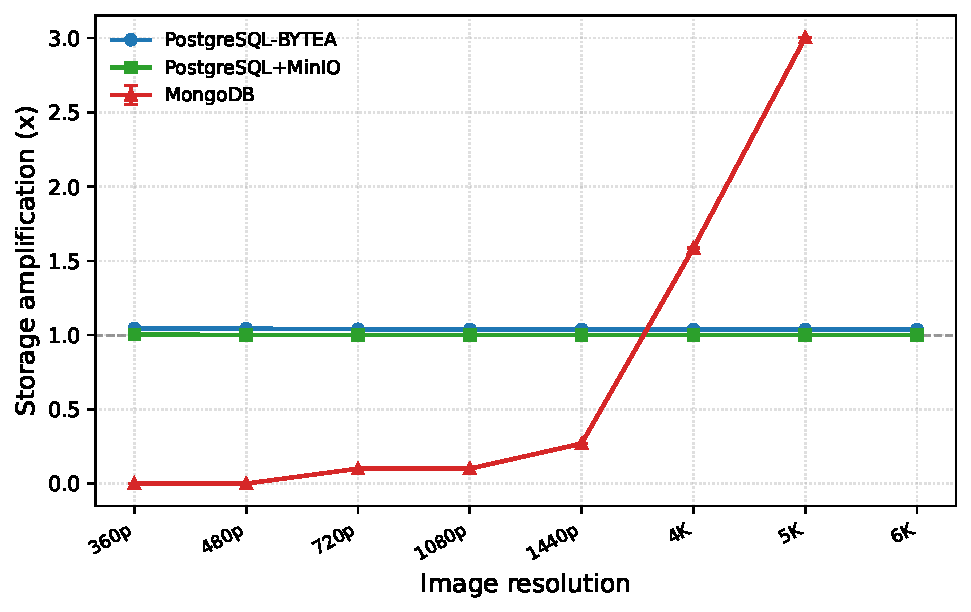
\includegraphics[width=\linewidth]{storage_amplification.pdf}
\caption{Storage amplification (disk space used $\div$ raw image size; the dashed line marks $1.0\times$, i.e.\ no overhead). PostgreSQL and the hybrid stay flat near $1.0\times$; MongoDB crosses from better-than-raw compression at low resolution to $3.0\times$ at 5K, with embodied-carbon consequences (Section~\ref{subsec:carbon}). MongoDB's values below 720p depend on the identical-row construction of the collage payload and rise substantially with real frames (Section~\ref{subsec:realframes}); the PostgreSQL and hybrid curves are unaffected, as neither compresses across rows. Unlike the other metrics, this figure is shown on a linear axis only: the logarithmic companion is omitted because storage amplification is a ratio read against $1.0\times$ and, for MongoDB, falls to zero at low resolution (0.000 at 480p, 0.001 at 360p)---values a logarithmic axis cannot represent, since the logarithm of zero is undefined.}\label{fig:storage}
\end{figure}

\begin{figure}[htbp]
\centering
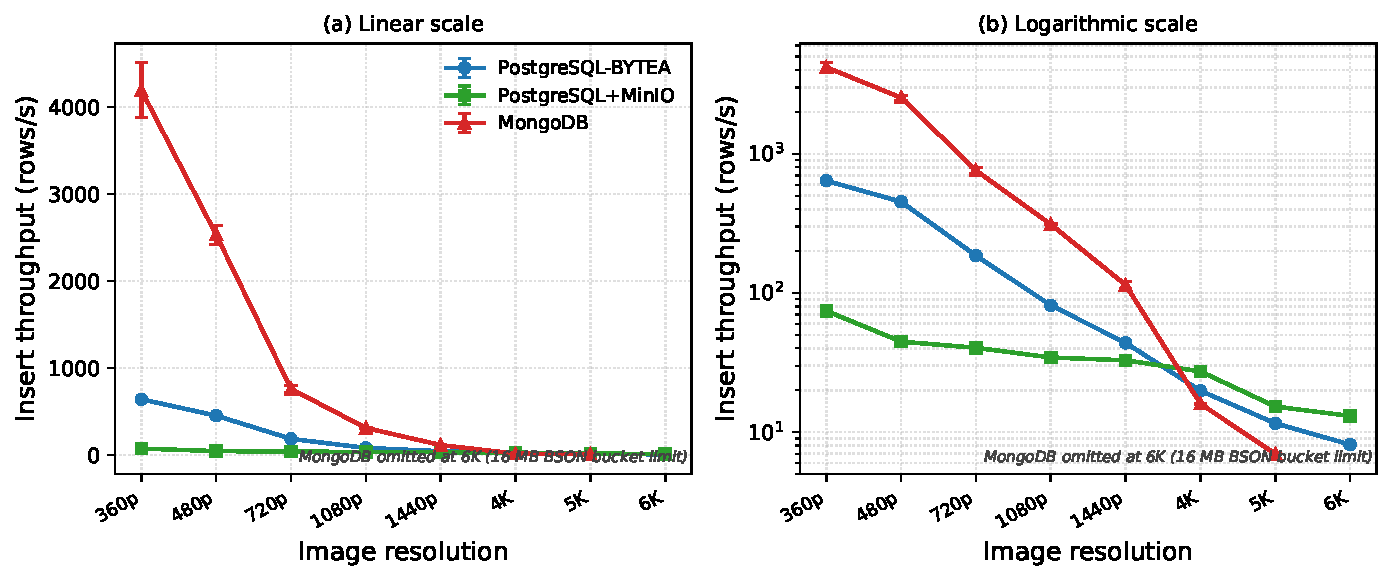
\includegraphics[width=\linewidth]{insert_throughput.pdf}
\caption{Insert throughput (records per second; mean$\pm$standard deviation over 5 runs), shown on a linear vertical axis (left) and a logarithmic one (right); the logarithmic panel makes the low-resolution behaviour visible. MongoDB dominates at low resolution but collapses at high resolution; the hybrid (PostMin) is flattest and leads from 4K. MongoDB is omitted at 6K (Section~\ref{subsec:bson}).}\label{fig:insert}
\end{figure}

\begin{table}[htbp]
\caption{Insert throughput (rows/s, mean$\pm$std) and storage amplification (on-disk $\div$ raw). Higher throughput and lower amplification are better; \textbf{bold} marks the best engine per row.}\label{tab:write}
\small
\setlength{\tabcolsep}{4pt}
\begin{tabular}{@{}lrrrrrr@{}}
\toprule
 & \multicolumn{3}{c}{Insert throughput (rows/s)} & \multicolumn{3}{c}{Storage amp. ($\times$)} \\
\cmidrule(lr){2-4}\cmidrule(lr){5-7}
Res. & Postgre & Mongo & PostMin & Postgre & Mongo & PostMin \\
\midrule
360p  & 640.9          & \textbf{4194.1} & 74.4          & 1.045 & \textbf{0.001} & 1.003 \\
480p  & 452.6          & \textbf{2532.4} & 44.7          & 1.044 & \textbf{0.000} & 1.002 \\
720p  & 185.7          & \textbf{760.3}  & 40.4          & 1.039 & \textbf{0.101} & 1.001 \\
1080p & 81.5           & \textbf{311.3}  & 34.4          & 1.039 & \textbf{0.101} & 1.000 \\
1440p & 43.8           & \textbf{114.2}  & 32.8          & 1.039 & \textbf{0.269} & 1.000 \\
4K    & 19.8           & 16.0            & \textbf{27.3} & 1.038 & 1.587 & \textbf{1.000} \\
5K    & 11.6           & 7.0             & \textbf{15.3} & 1.038 & 3.004 & \textbf{1.000} \\
6K    & 8.1            & --              & \textbf{13.1} & 1.038 & --    & \textbf{1.000} \\
\botrule
\end{tabular}
\footnotetext{Std deviations are small (e.g.\ MongoDB 360p $\pm$314; Postgre/PostMin typically $<2\%$). MongoDB at 6K is unstorable (Section~\ref{subsec:bson}).}
\end{table}

\subsection{Bulk retrieval and latest-frame reads}\label{subsec:retrieval}
Under a common workload across all three architectures, the read path tells the same mirror-image story (Figures~\ref{fig:retrieval}--\ref{fig:pointread}, Table~\ref{tab:read}). For \emph{bulk retrieval} of all 2{,}000 images, MongoDB's contiguous inline layout is fastest at low resolution (216~ms at 360p), but PostgreSQL degrades steeply as it pulls ever-larger \texttt{BYTEA} values out of out-of-line storage and through its client connection---reaching 53.6~s at 5K and 76.1~s at 6K. The hybrid is the most scalable reader: streaming objects over HTTP keeps bulk retrieval at 5.8~s (5K) and 8.6~s (6K), $9\times$ faster than inline PostgreSQL. \emph{Latest-frame reads} reinforce this: the hybrid stays near-flat (1--5~ms across the whole range) while PostgreSQL climbs to 39.6~ms at 6K and MongoDB to 69.8~ms at 5K. The hybrid is slightly slower than inline PostgreSQL only at the smallest resolutions, where its fixed HTTP round-trip (driver overhead 0.58~ms versus PostgreSQL's 0.05~ms) outweighs the streaming benefit.

\begin{figure}[htbp]
\centering
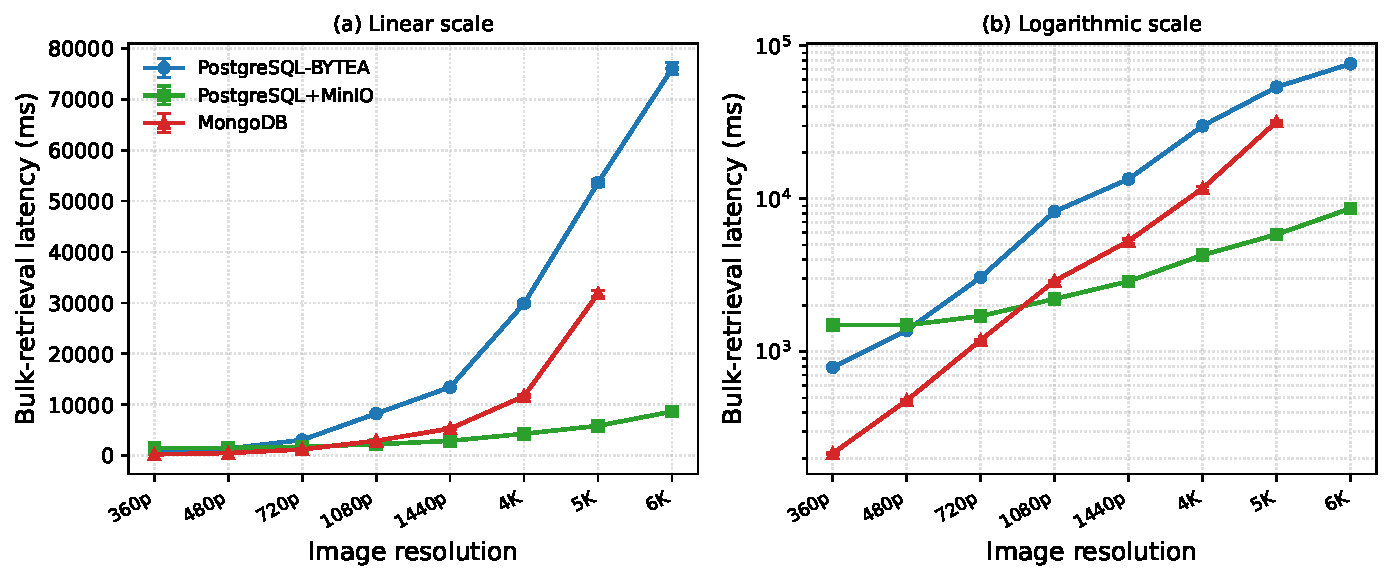
\includegraphics[width=\linewidth]{retrieval_latency.pdf}
\caption{Bulk-retrieval latency---the time to read back all 2{,}000 images in a range (milliseconds; mean$\pm$standard deviation), on linear (left) and logarithmic (right) axes. Inline PostgreSQL degrades steeply; the hybrid scales best.}\label{fig:retrieval}
\end{figure}

\begin{figure}[htbp]
\centering
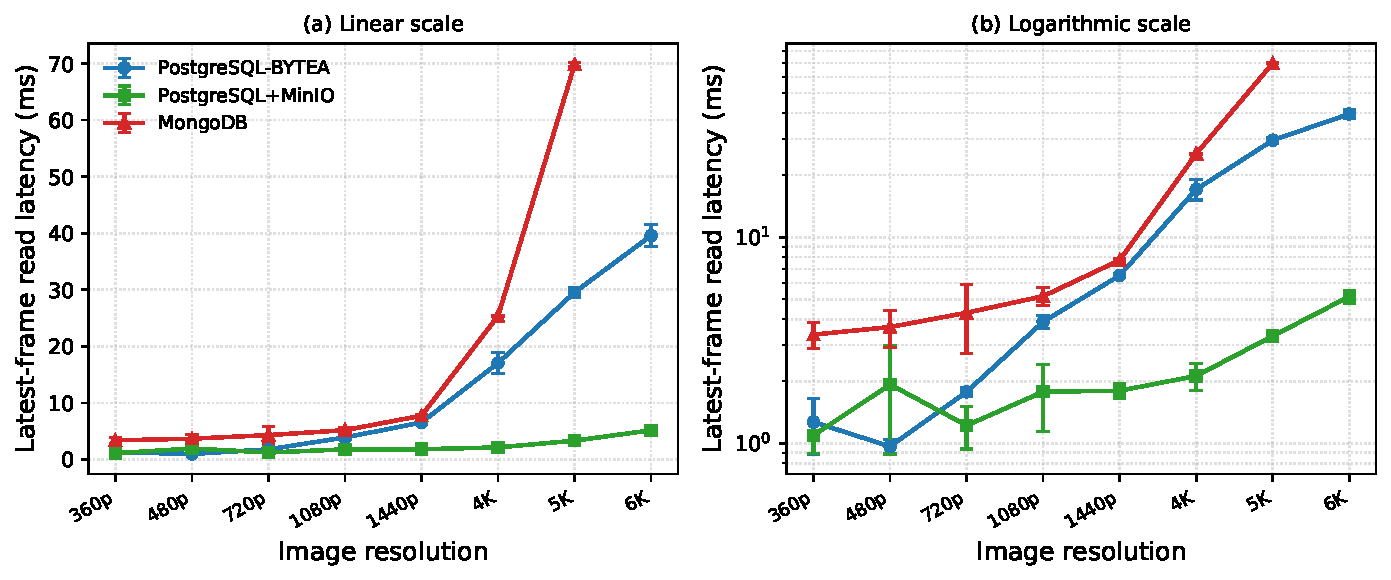
\includegraphics[width=\linewidth]{point_read_latency.pdf}
\caption{Latest-frame read latency---the time to fetch the single most recent image (milliseconds; mean$\pm$standard deviation), on linear (left) and logarithmic (right) axes. The hybrid stays near-flat; the inline architectures climb with image size.}\label{fig:pointread}
\end{figure}

\begin{table}[htbp]
\caption{Read latency (ms, mean$\pm$std): bulk retrieval of all 2{,}000 images, and the latest-frame read. Lower is better; \textbf{bold} marks the best architecture per row.}\label{tab:read}
\small
\setlength{\tabcolsep}{4pt}
\begin{tabular}{@{}lrrrrrr@{}}
\toprule
 & \multicolumn{3}{c}{Bulk retrieval (ms)} & \multicolumn{3}{c}{Latest-frame (ms)} \\
\cmidrule(lr){2-4}\cmidrule(lr){5-7}
Res. & Postgre & Mongo & PostMin & Postgre & Mongo & PostMin \\
\midrule
360p  & 788.5    & \textbf{215.9}  & 1497.2 & 1.27 & 3.37 & \textbf{1.09} \\
480p  & 1377.0   & \textbf{479.4}  & 1487.5 & \textbf{0.97} & 3.67 & 1.93 \\
720p  & 3057.7   & 1188.5 & \textbf{1706.9} & 1.78 & 4.30 & \textbf{1.22} \\
1080p & 8238.6   & 2895.8 & \textbf{2211.2} & 3.88 & 5.17 & \textbf{1.78} \\
1440p & 13433.1  & 5286.8 & \textbf{2879.9} & 6.52 & 7.74 & \textbf{1.80} \\
4K    & 29883.8  & 11669.3 & \textbf{4273.0} & 17.06 & 25.38 & \textbf{2.12} \\
5K    & 53638.4  & 31821.2 & \textbf{5833.4} & 29.55 & 69.83 & \textbf{3.31} \\
6K    & 76059.0  & --     & \textbf{8634.5} & 39.59 & --    & \textbf{5.15} \\
\botrule
\end{tabular}
\end{table}

\subsection{Carbon footprint per resolution}\label{subsec:carbon}
Table~\ref{tab:carbon} and Figure~\ref{fig:carbon} report directly measured per-resolution emissions and constitute the central result. Each value totals one insertion run, one bulk retrieval and one latest-frame read, weighting the three operations equally; Section~\ref{subsec:applied} shows how the selection changes under a write-dominated profile. They reveal a \emph{payload-dependent emission crossover with no universal winner}, in which MongoDB and the hybrid are mirror images and inline PostgreSQL is the pivot:
\begin{itemize}
  \item \textbf{Standard resolutions (360p--1440p): MongoDB is greenest}, and especially so at the low end---8~mg at 360p versus 38~mg (Postgre) and 187~mg (PostMin), a $4.8$--$23\times$ advantage---because near-empty compressed buckets ingest with little overhead. PostMin is the \emph{worst} here, penalised by a per-payload HTTP PUT on small images.
  \item \textbf{High resolutions (4K--6K): the hybrid is greenest}, emitting 526~mg at 4K and 1{,}023~mg at 5K---roughly half of inline PostgreSQL---by decoupling the multi-megabyte payload from the database write path. MongoDB is statistically indistinguishable from inline PostgreSQL at 4K (1{,}148 versus 1{,}128~mg, a $1.8\%$ gap that falls within insertion's run-to-run variability) and becomes \emph{clearly} the worst only at 5K (2{,}713~mg, $\approx 37\%$ above inline PostgreSQL) through inline BSON write amplification, defeated compression, and cache pressure, before failing entirely at 6K.
  \item \textbf{Inline PostgreSQL is the pivot}: it is never the greenest but operates across the whole range and avoids both extremes.
\end{itemize}
Insertion dominates the footprint (Figure~\ref{fig:breakdown}); bulk retrieval is the second contributor and latest-frame reads are negligible ($<1$~mg). Cumulatively over the common 360p--5K range, the hybrid is the lowest-carbon architecture at 3.13~g~CO\textsubscript{2}eq, $24.7\%$ below inline PostgreSQL (4.15~g) and $25.9\%$ below MongoDB (4.22~g): despite winning every standard resolution, MongoDB ends highest cumulatively because the high-resolution profiles dominate total energy. A CPU/RAM decomposition shows CPU accounts for $\approx$53\% of energy for the inline engines (Postgre, MongoDB) but only $\approx$41\% for the hybrid, consistent with PostMin offloading payload handling away from the database CPU path.

\begin{figure}[htbp]
\centering
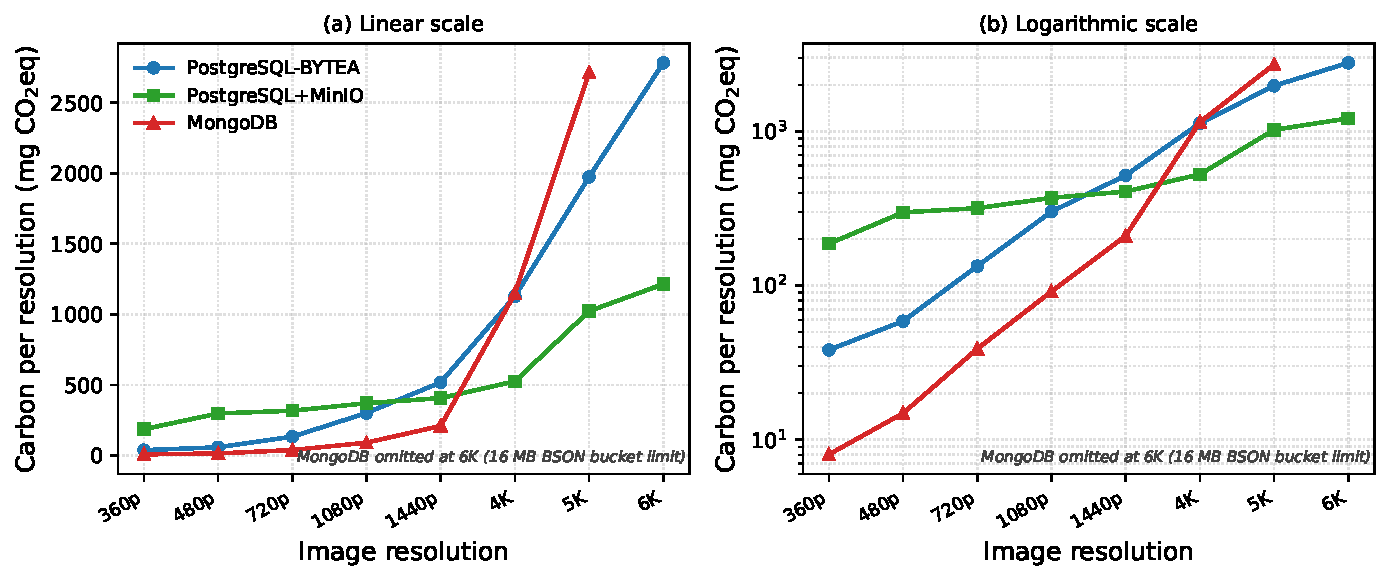
\includegraphics[width=\linewidth]{carbon_per_resolution.pdf}
\caption{Directly measured carbon per resolution (milligrams CO\textsubscript{2}eq; insertion + bulk retrieval + latest-frame read), on a linear axis (left) and a logarithmic one (right). The linear panel conveys the magnitude of the high-resolution emissions, while the logarithmic panel reveals the full ``scissors'' crossover: MongoDB is greenest at $\le$1440p, the hybrid greenest at $\ge$4K, and inline PostgreSQL the pivot. MongoDB is omitted at 6K (Section~\ref{subsec:bson}).}\label{fig:carbon}
\end{figure}

\begin{figure}[htbp]
\centering
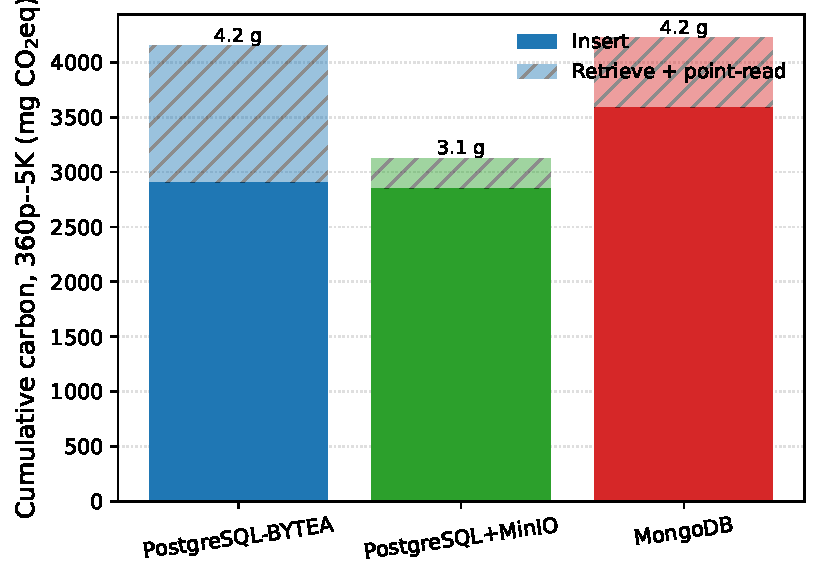
\includegraphics[width=0.85\linewidth]{carbon_breakdown.pdf}
\caption{Cumulative carbon over 360p--5K, split into insertion and read (bulk retrieval + latest-frame read) contributions. The hybrid is lowest overall; its read contribution is small because objects stream over HTTP rather than being pulled through the database.}\label{fig:breakdown}
\end{figure}

\begin{table}[htbp]
\caption{Directly measured carbon per resolution for one measured run: 2{,}000 inserts $+$ one 2{,}000-image bulk retrieval $+$ one latest-frame read (mg~CO\textsubscript{2}eq). Each tracker wrapped all five repeated runs, so every value is the integrated measurement divided by its run count. Lower is better; \textbf{bold} = greenest at that resolution.}\label{tab:carbon}
\small
\begin{tabular}{@{}lrrrl@{}}
\toprule
Res. & Postgre (BYTEA) & Mongo & PostMin (Postgre+MinIO) & Greenest \\
\midrule
360p  & 38.2    & \textbf{8.0}    & 186.6   & Mongo \\
480p  & 58.7    & \textbf{14.8}   & 298.2   & Mongo \\
720p  & 133.6   & \textbf{38.9}   & 317.6   & Mongo \\
1080p & 301.5   & \textbf{91.5}   & 370.5   & Mongo \\
1440p & 518.5   & \textbf{209.7}  & 407.0   & Mongo \\
4K    & 1128.0  & 1147.9 & \textbf{525.6} & PostMin \\
5K    & 1973.3  & 2712.9 & \textbf{1022.7} & PostMin \\
6K    & 2781.7  & --     & \textbf{1214.4} & PostMin \\
\midrule
\multicolumn{1}{@{}l}{Cum.\ 360p--5K} & 4151.8 & 4223.7 & \textbf{3128.2} & PostMin \\
\botrule
\end{tabular}
\footnotetext{Cumulative row over the common three-way range; MongoDB is highest cumulatively despite winning every standard resolution, because high-resolution profiles dominate total energy.}
\end{table}

\textbf{Software Carbon Intensity.} Expressing the storage operation in SCI terms~\citep{gsf_sci} with a functional unit of 1{,}000 stored frames (Table~\ref{tab:sci}), the carbon intensity of ingestion spans nearly three orders of magnitude across resolutions and inverts between engines: at 360p MongoDB stores 1{,}000 frames for 2.7~mg~CO\textsubscript{2}eq versus 83.6~mg for the hybrid, whereas at 5K the hybrid needs 467~mg versus MongoDB's 1{,}167~mg. SCI makes the operating-point dependence explicit and portable across deployments.

\begin{table}[htbp]
\caption{Software Carbon Intensity of ingestion: mg~CO\textsubscript{2}eq per 1{,}000 stored frames (Indonesian grid). Lower is better.}\label{tab:sci}
\small
\begin{tabular}{@{}lrrr@{}}
\toprule
Res. & Postgre & Mongo & PostMin \\
\midrule
360p  & 13.6   & \textbf{2.7}   & 83.6 \\
480p  & 20.0   & \textbf{4.4}   & 139.1 \\
720p  & 47.0   & \textbf{12.3}  & 147.4 \\
1080p & 103.4  & \textbf{28.8}  & 170.6 \\
1440p & 184.0  & \textbf{75.4}  & 184.0 \\
4K    & 399.3  & 506.2  & \textbf{232.0} \\
5K    & 686.1  & 1166.8 & \textbf{466.6} \\
6K    & 963.4  & --     & \textbf{542.6} \\
\botrule
\end{tabular}
\end{table}

\textbf{Carbon of the read operations.} The same crossover recurs within each read operation (Table~\ref{tab:dimcarbon}). For bulk retrieval, MongoDB is greenest up to 720p and the hybrid from 1080p---an earlier crossover than insertion, because the hybrid's HTTP streaming avoids pulling large values through the database engine. Latest-frame reads cost under 1~mg throughout and are led by the hybrid wherever the workload is non-trivial. Because insertion (Table~\ref{tab:sci}) is the dominant contributor, these per-operation winners carry through to the totals in Table~\ref{tab:carbon}.

\begin{table}[htbp]
\caption{Carbon of the two read operations (mg~CO\textsubscript{2}eq per single run: one 2{,}000-image bulk retrieval or one latest-frame read), completing the per-operation breakdown alongside insertion (Table~\ref{tab:sci}) and the total (Table~\ref{tab:carbon}). Lower is better; \textbf{bold} = greenest per row.}\label{tab:dimcarbon}
\small
\setlength{\tabcolsep}{4pt}
\begin{tabular}{@{}lrrrrrr@{}}
\toprule
 & \multicolumn{3}{c}{Bulk retrieval (mg)} & \multicolumn{3}{c}{Latest-frame (mg)} \\
\cmidrule(lr){2-4}\cmidrule(lr){5-7}
Res. & Postgre & Mongo & PostMin & Postgre & Mongo & PostMin \\
\midrule
360p  & 11.0   & \textbf{2.6}   & 19.4  & 0.04 & \textbf{0.03} & 0.05 \\
480p  & 18.8   & \textbf{6.0}   & 19.8  & 0.05 & \textbf{0.03} & 0.06 \\
720p  & 39.5   & \textbf{14.2}  & 22.8  & 0.06 & \textbf{0.05} & 0.06 \\
1080p & 94.5   & 33.8 & \textbf{29.2} & 0.09 & 0.08 & \textbf{0.06} \\
1440p & 150.4  & 58.9 & \textbf{38.9} & 0.13 & 0.11 & \textbf{0.06} \\
4K    & 329.2  & 135.2 & \textbf{61.6} & 0.25 & 0.32 & \textbf{0.07} \\
5K    & 600.7  & 378.5 & \textbf{89.4} & 0.39 & 0.88 & \textbf{0.09} \\
6K    & 854.4  & --    & \textbf{129.1} & 0.51 & --  & \textbf{0.11} \\
\botrule
\end{tabular}
\footnotetext{Latest-frame carbon is negligible in absolute terms ($<1$~mg); the hybrid leads it from 1080p upward, with MongoDB marginally lower only where all three are near zero.}
\end{table}

\textbf{Embodied carbon of storage amplification.} Operational energy is not the only cost: provisioned storage carries embodied (manufacturing) carbon~\citep{gupta_chasing_carbon,tannu_ssd_embodied}. At 5K, 2{,}000 frames occupy $10.7$~GB of raw payload; the hybrid provisions essentially that, inline PostgreSQL $\approx$11.1~GB, and MongoDB's $3.00\times$ amplification $\approx$32.0~GB. Capacities are stated in decimal gigabytes throughout, matching the convention in which storage devices are sold and in which the embodied intensity is expressed. Using a representative NAND-flash embodied intensity of 0.16~kg~CO\textsubscript{2}eq/GB~\citep{tannu_ssd_embodied}, MongoDB carries $\approx$5.1~kg of embodied carbon for this data versus $\approx$1.7~kg for the hybrid---a one-time $\approx$3.4~kg penalty that recurs with every retained dataset and compounds at fleet scale through faster device wear. This is deliberately a first-order, single-factor estimate: it applies one representative cell-level NAND intensity to the \emph{storage medium only}---excluding controller, DRAM, packaging, transport, and end-of-life stages---and assumes embodied carbon scales linearly with provisioned capacity, so it conveys the order of magnitude and the \emph{direction} of the amplification penalty rather than a full life-cycle assessment; a complete LCA with device-specific boundaries is left to future work.

\subsection{Multi-region grid-intensity sensitivity}\label{subsec:grid}
\emph{Grid carbon intensity} is the mass of CO\textsubscript{2}eq released per unit of electricity generated, and it varies widely by region---from a few tens of grams per kilowatt-hour on hydro- or nuclear-dominated grids to over 700 on coal-heavy ones~\citep{owid_carbon_intensity}. The same computation therefore emits very different amounts of carbon depending on where it runs. A \emph{multi-region grid-intensity sensitivity} analysis re-evaluates the carbon footprint under several such regional grids to test how robust the conclusions are to the deployment location. Because emissions equal energy times grid intensity, the architecture \emph{ranking} is grid-invariant while the \emph{absolute} footprint scales with the local grid (Table~\ref{tab:grid}). Recomputing the cumulative 360p--5K footprint across representative national grids~\citep{owid_carbon_intensity} from near-decarbonised (Sweden, 41~g/kWh) to coal-heavy (India, 713~g/kWh), the hybrid remains the lowest-carbon choice everywhere, and the absolute saving versus MongoDB grows from 0.066~g (Sweden) to 1.16~g (India) for this modest 2{,}000-frame-per-resolution workload. Grid decarbonisation shrinks the absolute stakes but does not change which architecture an operator should choose. We therefore present this sweep as a bounding exercise---a linear rescaling of one measured energy figure---rather than an independent finding. The carbon-specific results that do \emph{not} reduce to operational energy are the embodied-carbon penalty of storage amplification (Section~\ref{subsec:carbon}), which scales with provisioned capacity rather than runtime, and the operating-point inversion made explicit by Software Carbon Intensity; these are where the carbon lens adds information beyond a conventional energy benchmark.

\begin{table}[htbp]
\caption{Multi-region grid sensitivity: cumulative footprint over 360p--5K (g~CO\textsubscript{2}eq) under different grid intensities, counting one insertion, one bulk retrieval, and one latest-frame read equally. The hybrid (PostMin) has the lowest cumulative total under every grid.}\label{tab:grid}
\small
\begin{tabular}{@{}lrrrr@{}}
\toprule
Grid region & g/kWh & Postgre & Mongo & PostMin \\
\midrule
Sweden            & 41  & 0.25  & 0.26  & \textbf{0.19} \\
France            & 53  & 0.33  & 0.33  & \textbf{0.25} \\
EU-27 average     & 230 & 1.41  & 1.44  & \textbf{1.06} \\
United States     & 360 & 2.21  & 2.25  & \textbf{1.67} \\
China             & 550 & 3.38  & 3.44  & \textbf{2.55} \\
Indonesia$^\ast$  & 676 & 4.15  & 4.22  & \textbf{3.13} \\
India             & 713 & 4.38  & 4.45  & \textbf{3.30} \\
\botrule
\end{tabular}
\footnotetext{$^\ast$Baseline grid used for all other tables. Grid intensities are representative national values~\citep{owid_carbon_intensity}; exact figures vary by year and data source.}
\end{table}

\subsection{The MongoDB 16~MiB ceiling}\label{subsec:bson}
MongoDB could not store 6K frames at all. The 6K payload is 7.13~MB---comfortably within the 16~MiB BSON document limit for a single frame---yet insertion failed with error~10334 (\texttt{BSONObjectTooLarge}), the offending object measuring 22.4~MB ($\approx$3$\times$ the payload). The cause is architectural: native Time-Series Collections \emph{bucket} multiple measurements that share a metadata value into a single underlying bucket document, which is itself bound by the 16~MiB BSON limit. With multi-megabyte payloads only two frames fit in a bucket; the attempt to bucket a third breaches the ceiling. The same bucketing that makes time-series collections efficient for small measurements becomes a hard limit for large binaries, and---unlike a tuning parameter---it cannot be raised. Two things should be separated here. The 16~MiB ceiling on a single BSON document is fixed by the specification, and no configuration or hardware raises it. Whether several frames are combined into one document that exceeds it, however, depends on how the collection is configured: we use the default bucketing of a native time-series collection with a single metadata value shared by every row, which is the configuration a practitioner adopting time-series collections would obtain without deliberate tuning. Under that configuration \emph{MongoDB inline storage is not merely inefficient but infeasible} at 6K, and no cache setting or larger machine changes it. A different bucket span or a higher metadata cardinality would place fewer frames in each bucket and might postpone the failure, which we did not test. A second and quite different limit, which does depend on the host, is reported in Section~\ref{subsec:memory}.

\subsection{The same payloads on two machines}\label{subsec:twohosts}
The measurements above come from one computer. Repeating the entire collage sweep on a second, markedly smaller machine tests whether the ordering and its crossover are properties of the architectures or of the host. The payload sizes are identical in both columns of Table~\ref{tab:twohosts}, as are the database images and the benchmark protocol. The environments are not identical in every respect: the operating-system point release, container runtime, Python patch level, and storage device differ as well as the processor and memory (Table~\ref{tab:env2}). We therefore attribute the difference to the environment rather than to the processor alone, while noting that the components held constant are the ones that determine how each architecture handles the payload.

Three things follow. The \textbf{ordering at small payloads is unchanged}: MongoDB has the lowest ingestion carbon at every payload up to $0.80$~MB on both machines, so the low-payload conclusion does not depend on the host. MongoDB's \textbf{advantage is exhausted earlier} on the smaller environment. At $1.40$~MB it emits $0.41\times$ the hybrid's amortised ingestion carbon on the larger machine, a clear margin, but $1.01\times$ on the smaller, where the two are within $1\%$ of one another. We do not read that as establishing a crossover at $1.40$~MB: a $1\%$ separation is well inside the run-to-run variability of that environment, and each carbon value is a single integrated measurement. What the pair does establish is that a margin of more than a factor of two on one machine has disappeared on the other at the same payload, which is larger than the variability and is the direction the mechanism predicts, since the hybrid's benefit is keeping bytes out of the database write path and a smaller host is where that path is most constrained.

Third, and not anticipated, \textbf{MongoDB ceases to be runnable} on the smaller machine from 4K upward, for reasons reported in Section~\ref{subsec:memory}, while inline PostgreSQL and the hybrid complete every payload to $7.13$~MB on the same host in the same session.

\begin{table}[htbp]
\caption{The same collage payloads measured on two environments. Values are the amortised ingestion carbon in mg~CO\textsubscript{2}eq per frame; \textbf{bold} marks the lowest in each row, except where the two are within measurement variability. Payload sizes, database images, and protocol are held constant; processor, memory, storage, operating-system point release, container runtime, and Python patch level all differ (Table~\ref{tab:env2}).}\label{tab:twohosts}
\small
\setlength{\tabcolsep}{4pt}
\begin{tabular}{@{}lr rrr rrr@{}}
\toprule
 & & \multicolumn{3}{c}{i9, 16 threads, 31~GB} & \multicolumn{3}{c}{i7, 8 threads, 15~GB} \\
\cmidrule(lr){3-5}\cmidrule(lr){6-8}
Resolution & MB & Postgre & PostMin & Mongo & Postgre & PostMin & Mongo \\
\midrule
360p  & 0.09 & 0.0136 & 0.0836 & \textbf{0.0027} & 0.0087 & 0.0277 & \textbf{0.0020} \\
480p  & 0.16 & 0.0200 & 0.1391 & \textbf{0.0044} & 0.0146 & 0.0431 & \textbf{0.0049} \\
720p  & 0.36 & 0.0470 & 0.1474 & \textbf{0.0123} & 0.0314 & 0.0608 & \textbf{0.0184} \\
1080p & 0.80 & 0.1034 & 0.1706 & \textbf{0.0288} & 0.0748 & 0.0928 & \textbf{0.0365} \\
\midrule
1440p & 1.40 & 0.1840 & 0.1840 & \textbf{0.0754} & 0.1889 & 0.1274 & 0.1287 \\
4K    & 2.99 & 0.3993 & \textbf{0.2320} & 0.5062 & 0.4401 & \textbf{0.2186} & failed \\
5K    & 5.09 & 0.6861 & \textbf{0.4666} & 1.1668 & 0.7730 & \textbf{0.4024} & --- \\
6K    & 7.13 & 0.9634 & \textbf{0.5426} & failed & 1.1198 & \textbf{0.4659} & --- \\
\botrule
\end{tabular}
\footnotetext{The horizontal rule marks where the two machines diverge: above it the ordering is identical, below it the hybrid takes over one payload step earlier on the smaller machine. ``failed'' denotes a cell attempted and terminated, MongoDB at 6K by the BSON ceiling (Section~\ref{subsec:bson}) and at 4K on the smaller host by memory exhaustion (Section~\ref{subsec:memory}); ``---'' denotes a cell not attempted, the run having ended at that point. Run-to-run variability is higher on the smaller machine, reaching a coefficient of variation of $28\%$ against under $6\%$ on the larger, which is why we report the direction and magnitude of the shift rather than a precise crossover payload for it.}
\end{table}

\subsection{A second infeasibility: memory, not protocol}\label{subsec:memory}
Section~\ref{subsec:bson} reports a limit that no hardware raises: under the tested time-series configuration, bucketed documents breach the 16~MiB BSON ceiling at 6K. Repeating the measurements on the smaller host revealed a second limit, of a different kind, and it is worth reporting because a practitioner will meet it long before the first.

On the 15.30~GB host, MongoDB completed 360p through 1440p and then stopped being runnable. Its ingest rate on that host falls steeply with payload, from $3{,}973$~rows/s at 360p to $28.9$~rows/s at 1440p, and at 4K it collapsed to between three and five rows per second, roughly a thousandfold below its low-resolution rate. The insertion then terminated with the client reporting a broken connection. The system journal records the cause: the kernel invoked the out-of-memory killer against the \texttt{mongod} process twice, under a global memory constraint rather than a container limit. The cell was retried once, killed again, and recorded as skipped. Inline PostgreSQL and the hybrid completed every resolution to 6K on the same host, in the same session, without incident.

The mechanism follows directly from how the architectures place the payload. WiredTiger keeps documents uncompressed in cache, so one insertion run of 2{,}000 frames at 4K constitutes $5.8$~GB of live working set that quality-90 JPEG gives it no way to shrink. PostgreSQL relocates the same payload out of line through TOAST, and the hybrid never admits it to the database at all, so neither accumulates a comparable resident set. What is a tuning parameter at small payloads becomes, at large ones, the difference between an architecture that runs and one that does not.

Two qualifications belong with this. The cache was configured at $14$~GB, the same proportion of host memory as the $30$~GB used on the larger machine, so the ratio was held constant rather than the absolute size; and the host carried no swap, so memory pressure produced termination rather than degradation. A more conservative cache would likely have completed the sweep more slowly. That, however, is the point: the configuration that is unremarkable on a well-provisioned host is not survivable on a modest one, and it is MongoDB alone among the three that is sensitive to the difference. For an operator choosing a store for large images on constrained hardware, whether an architecture runs at all is a more immediate consideration than the margins between those that do.

\subsection{Reinforcing the results with a real-case deployment}\label{subsec:realframes}
The benchmark above builds one deterministic collage per resolution and inserts it for every row, so all 2{,}000 stored rows are byte-identical. That construction is exactly reproducible, which is what a controlled comparison requires, but it is not what a camera produces: identical rows are compressible in a way real data is not. We therefore reinforce the controlled results with a real-case deployment: a corpus of real frames recorded from a \emph{face-recognition-based attendance system} in operational use, an installation that captures images from one networked camera and two USB cameras in order to identify people at entry, over which the benchmark is run again with a different real image for every inserted row. The deployment is of exactly the class this paper addresses, retaining image streams alongside timestamped metadata in a continuously running data tier. What we take from it is the \emph{storage} workload: the images its cameras produce, at the resolutions and capture rate the installation actually uses. The recognition pipeline itself, meaning face detection, embedding, matching, and their accuracy and energy cost, lies outside the scope of this paper, which is concerned with the carbon cost of retaining the images rather than of analysing them. That boundary matters for reading the results: the figures reported here are those of the data tier alone, and a deployment's total footprint would additionally include the inference workload we do not measure. The cameras and the capture regime are those of the deployment; the benchmark itself was then executed on the hosts of Table~\ref{tab:env2}, so the deployment supplies the \emph{workload} while the storage measurements remain on controlled, fully specified hardware. Ten minutes of capture at 5~frames per second yielded 2{,}845--2{,}988 frames per camera; every frame was verified byte-distinct, and an automated sweep detected no faces in any of them (see the ethics statement for what that does and does not establish).

The deployment is characterised in Table~\ref{tab:deployment}. It is a heterogeneous installation of the kind the decision framework is intended for, and its capture regime is set by the recognition task rather than by storage considerations: one networked camera delivering H.264 video over RTSP (Real-Time Streaming Protocol, the protocol by which network cameras deliver a continuous video stream) and two USB cameras delivering Motion JPEG (MJPG, in which every frame is an independently compressed JPEG image), differing in native resolution and, as the table shows, in the payload each produces at a given resolution. That heterogeneity is itself a finding. At an identical 1080p the two cameras differ by 12\% in encoded size, and the direction reverses at 720p, because the networked camera's additional bytes sit in high-frequency content that downscaling removes. Payload size is therefore not determined by the resolution a camera advertises, which is a further reason to key the decision rule (Section~\ref{subsec:model}) to measured payload size rather than to a nominal resolution.

\textbf{The capture application.} Because the corpus must be reproducible by others, the recorder is provided with the artifact and specified here. It is a small application, of the kind an operator of such a deployment would actually run, and its design choices matter to the measurements it produces.

Each camera is read by an independent worker thread that pulls frames continuously and retains only the most recent one. Reading continuously is not an optimisation but a correctness requirement for the networked camera: a client that reads intermittently allows unread frames to accumulate inside the stream, and the recording drifts progressively behind real time. Frames are then retained at a configured rate rather than at the rate the camera delivers, because the cameras ignore a request to run slower; the application therefore reads every frame and keeps every $n$th, which is the only way to record a chosen rate faithfully. USB cameras are opened in Motion JPEG mode deliberately: in the uncompressed alternative the bus limits 1080p capture to roughly 10~frames per second, whereas in-camera compression sustains 30. Each retained frame is encoded once, at the same quality~90 used for the collage payloads, so that the two corpora remain comparable.

Two properties of the corpus follow from the design rather than from inspection after the fact. Every frame is independently captured and encoded, so no two rows share content, which is precisely the property the single-image collage lacks. And a face detector is run over every saved frame at the end of a recording session, reporting any frame in which a face is found, so that a corpus intended for release is verified rather than assumed to be free of personal data.

\begin{table}[htbp]
\caption{The face-recognition-based attendance system used as the real-case deployment. Frames were captured simultaneously from all three cameras for ten minutes at 5~frames per second. ``Recorded size'' is the mean encoded size of the frames \emph{as captured}, with standard deviation, at each camera's native resolution. It is not the payload the benchmark stores: frames are resized to the target profile and re-encoded before measurement, which changes their size, and the benchmark's payload figures are reported separately in Section~\ref{subsec:realframes}. The external USB camera is the only one of the three able to capture 1080p; the built-in camera's sensor is limited to $1280\times720$.}\label{tab:deployment}
\small
\begin{tabular}{@{}llrrr@{}}
\toprule
Camera & Transport & Native resolution & Frames & Recorded size (KB) \\
\midrule
Networked (IP) & H.264 / RTSP & $1920\times1080$ & 2{,}845 & $163.5\pm1.3$ \\
USB, external  & Motion JPEG  & $1920\times1080$ & 2{,}988 & $156.7\pm0.2$ \\
USB, built-in  & Motion JPEG  & $1280\times720$  & 2{,}891 & $\phantom{0}69.3\pm0.3$ \\
\botrule
\end{tabular}
\footnotetext{All 8{,}724 frames were verified byte-distinct, and every frame was checked automatically for the presence of a face before use; none was found. The capture rate of 5~frames per second is the installation's own operating setting. We note in passing that a higher rate would multiply stored frames, and hence storage carbon, in direct proportion; whether it would improve recognition is a question about the inference pipeline and is not evaluated here.}
\end{table}

Three findings follow (Table~\ref{tab:realframes} and Figure~\ref{fig:realframes}). First, \textbf{the architectural conclusion holds under the equal-weight profile}: counting one insertion, one bulk retrieval and one latest-frame read equally, MongoDB is the lowest-carbon architecture at every resolution from 360p to 1080p, exactly as the collage sweep reports for this range, and the result replicates independently on a second camera. Second, \textbf{real payloads are far smaller than the single-image collage}, by $3.1\times$ at 360p rising to $5.4\times$ at 1080p, confirming that the quality-90 collage is close to a worst case for compressibility rather than a typical one. Third, and most consequential, \textbf{storing one repeated image rather than distinct ones materially overstates MongoDB's advantage}. Comparing at approximately matched payload size on the same environment (Table~\ref{tab:repetition}), all three architectures change, but only MongoDB changes for the worse: its amortised ingestion carbon rises by $2.4$ to $2.9\times$ and its storage amplification by $16$ to $25\times$, while PostgreSQL and the hybrid become cheaper. The asymmetry has a single cause: MongoDB is the only one of the three that compresses \emph{across} rows, bucketing many frames into one document in which Snappy removes repeated content almost entirely. TOAST compresses per value and MinIO stores per object, so neither benefits from repetition and neither is distorted by it.

The two corpora therefore agree on \emph{which} architecture to choose over most of the range and differ on \emph{by how much}, with the difference traceable to a single mechanism. With realistic payloads MongoDB's margin narrows sharply as resolution rises, and the crossover to the hybrid is correspondingly expected earlier than the 1440p--4K interval observed under the collage workload. We accordingly read the two together: the collage sweep establishes the ordering across the full 360p--6K range, where only it can reach, and the real-case corpus establishes the magnitude that a practitioner should expect from ordinary camera output. Two caveats bound the comparison: real frames differ from the collage in size as well as in distinctness, so the two effects are not fully separable; and bucket packing itself depends on absolute payload size. The matched-size comparison above is the cleanest available attribution, not a controlled isolation of a single variable.

\begin{figure}[htbp]
\centering
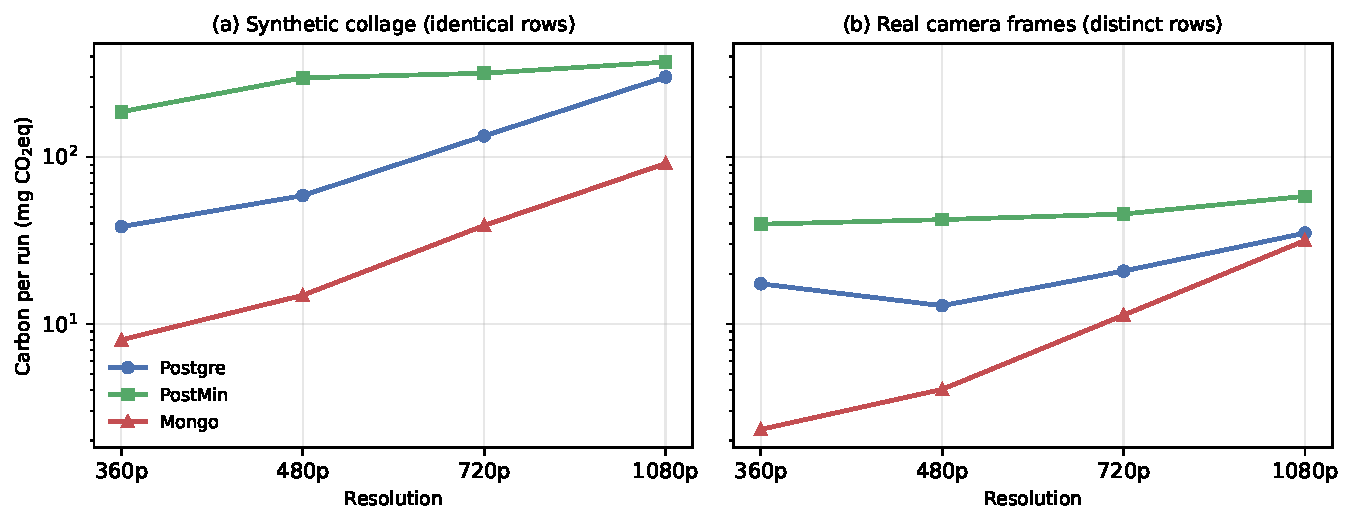
\includegraphics[width=\linewidth]{realframes_carbon.pdf}
\caption{Carbon per run against resolution, with the single-image collage (a) beside real recorded camera frames (b). Note the logarithmic vertical axis. The engine ordering is identical in both panels, with MongoDB lowest throughout the measured range under the equal-weight profile, which is the result that validates the study's conclusion. The panels differ in the \emph{spread} between architectures: with identical rows (a) MongoDB's margin over inline PostgreSQL is wide and grows, whereas with distinct real frames (b) the two converge as resolution rises, and are within 11\% at 1080p. The identical-row construction therefore preserves the ordering but exaggerates the margin.}\label{fig:realframes}
\end{figure}

\begin{table}[htbp]
\caption{Real recorded camera frames versus the single-image collage, 360p--1080p, on the networked camera. Carbon is the per-run total of insertion, bulk retrieval, and latest-frame read. ``Amp'' is MongoDB's storage amplification. Every row of the real-frame runs receives a different photograph.}\label{tab:realframes}
\small
\begin{tabular}{@{}lrrrrrr@{}}
\toprule
 & \multicolumn{2}{c}{Payload (MB)} & \multicolumn{2}{c}{Mongo carbon (mg)} & \multicolumn{2}{c}{Mongo amp ($\times$)} \\
\cmidrule(lr){2-3}\cmidrule(lr){4-5}\cmidrule(lr){6-7}
Resolution & Collage & Real & Collage & Real & Collage & Real \\
\midrule
360p  & 0.09 & 0.03 &  8.03 &  2.33 & 0.001 & 0.000 \\
480p  & 0.16 & 0.05 & 14.84 &  4.05 & 0.000 & 0.000 \\
720p  & 0.36 & 0.09 & 38.85 & 11.28 & 0.101 & \textbf{0.274} \\
1080p & 0.80 & 0.15 & 91.46 & 31.59 & 0.101 & \textbf{0.924} \\
\botrule
\end{tabular}
\footnotetext{Under the equal-weight profile MongoDB has the lowest total in every row of both runs, and on the second camera as well: at 1080p the three real-frame totals are $31.59$ (Mongo), $34.99$ (Postgre), and $58.17$~mg on this camera, and $18.82$, $29.94$, and $90.42$~mg on the external USB camera. Under an ingestion-only profile the 1080p ordering reverses to inline PostgreSQL (Section~\ref{subsec:applied}). Storage amplification for PostgreSQL ($1.03$--$1.09\times$) and the hybrid ($1.00$--$1.02\times$) is unchanged by payload realism, as expected: neither compresses across rows.}
\end{table}

The real-case runs were executed on a \emph{different computer} from the controlled benchmark (Table~\ref{tab:env2}), so they vary hardware as well as payload. The validation host is an ultraportable-class Intel Core i7-1165G7 with four physical cores, against the eight-core mobile-workstation Core i9-11900H used for the controlled benchmark: half the cores, half the memory, and a proportionally scaled MongoDB cache of 14~GB in place of 30~GB. Absolute figures differ between the two machines, as they must. The ordering does not change between the experiments we ran, which is what the mechanism of Section~\ref{subsec:model} implies: the crossover is driven by the ratio of fixed to per-byte cost rather than by absolute speed, so halving the core count and the cache rescales both terms without reordering them. That is weaker than hardware independence, and we claim no more. The real corpus was measured on this host only, and the collage comparison of Section~\ref{subsec:twohosts} varied the operating-system point release, container runtime, and Python patch level alongside the processor and memory. What the pair establishes is consistency across the tested host and corpus combinations.

\begin{table}[htbp]
\caption{The second environment used for the real-frame validation, beside the environment of the controlled benchmark. The two differ in processor class, core count, and memory, so agreement between them is stronger evidence than a repeated measurement on one machine; they also differ in operating-system point release, container runtime, and Python patch level, so the comparison does not isolate the processor.}\label{tab:env2}
\small
\begin{tabular}{@{}lll@{}}
\toprule
Component & Controlled benchmark & Real-case host \\
\midrule
CPU & Core i9-11900H, 8C/16T & Core i7-1165G7, 4C/8T \\
    & 2.50--4.90~GHz & 2.80--4.70~GHz \\
RAM & 30.99~GB & 15.30~GB \\
SSD & 1.9~TB Samsung NVMe & 477~GB Samsung NVMe \\
OS & Ubuntu 24.04.4 LTS & Ubuntu 24.04.3 LTS (Linux 6.8.0) \\
Containers & Docker 29.4.0, Compose v5.1.1 & Docker 29.7.2, Compose v5.4.0 \\
MongoDB cache & 30~GB & 14~GB$^{\ddagger}$ \\
Runtime & Python 3.14 & Python 3.14.7, CodeCarbon 3.2.7 \\
\botrule
\end{tabular}
\footnotetext{Database images are identical in both environments: TimescaleDB \texttt{latest-pg15}, MongoDB 7.0, MinIO \texttt{latest}. The MongoDB cache is set to the same near-total fraction of host memory in each case ($\approx$97\% and $\approx$92\%), so that WiredTiger's behaviour under memory pressure, which drives its high-resolution collapse, is preserved rather than altered. $^{\ddagger}$Holding that proportion constant is what makes the two environments comparable, but on the smaller host it left no headroom: see Section~\ref{subsec:memory}. Neither host was configured with swap.}
\end{table}

\subsection{Payload size, not resolution, determines the outcome}\label{subsec:sizevsres}
The results so far have been indexed by resolution, which is how a camera is specified and how an operator would naturally state a requirement. Taken together, however, the two corpora show that resolution is a label for the deciding variable rather than the variable itself, and that the substitution fails in practice and not merely in principle.

Three observations establish this, and the third settles it.

\textbf{The same resolution produces very different payloads.} A 1080p frame is $0.804$~MB as a quality-90 collage and $0.149$~MB as ordinary camera output, a factor of $5.4$; across 360p to 1080p the factor runs from $3.1$ to $5.4$. The collage is high-entropy by construction and close to a worst case for compressibility, whereas a real scene is not, and no resolution label distinguishes the two.

\textbf{Even two real cameras disagree at the same resolution.} The networked camera and the higher-specified USB camera differ by $12.3$\% in encoded size at 1080p, and the sign of that difference reverses at 720p, where the USB camera produces the larger payload. The reason is spectral rather than nominal: the networked camera delivers H.264 and carries more high-frequency content, which survives at native resolution and is removed by downscaling. Two cameras sold as the same resolution therefore sit at different points on the payload axis, and their order can invert between resolutions.

\textbf{The consequence is a different architecture, not merely a different number.} At 1080p on one host, and under an ingestion-only profile, the collage payload selects MongoDB and real camera output selects inline PostgreSQL. The resolution is identical, the machine is identical, the software is identical, and the recommendation is opposite. The second camera corroborates this and sharpens it: its 1080p output is $0.131$~MB and still selects MongoDB, whereas the first camera's $0.149$~MB does not, so the two together place the transition between those payloads. Neither camera alone brackets it that closely, and both are labelled 1080p. An operator applying a resolution-banded rule to a camera whose output is lighter than the rule's calibration would adopt the architecture that is not the greenest for their workload.

We therefore state the decision rule in Section~\ref{sec:framework} in terms of measured payload size, and treat resolution as an indicative guide whose reliability is specific to the camera and the scene. This is not a refinement of presentation. A rule expressed in resolutions is wrong for any deployment whose cameras produce payloads unlike those used to calibrate it, which, as the first observation shows, is the common case rather than the exceptional one.

%%=====================================================================%%
\section{A Carbon-Aware Decision Framework}\label{sec:framework}
%%=====================================================================%%

\subsection{Which architecture wins each operation}\label{subsec:winners}
Two regularities across the four operations motivate a single decision rule. First, for the two operations that dominate the footprint---insertion and bulk retrieval---the lowest-carbon architecture is also the fastest at every payload measured, because those operations are long enough that elapsed time dominates and energy is power integrated over time. The correspondence is not universal, however, and we do not claim it as such. For latest-frame reads it fails: at 360p and 720p the hybrid returns the frame fastest while MongoDB emits least, and at 480p inline PostgreSQL is fastest while MongoDB is again the greenest. A point read completes in one to two milliseconds, so differences in average power during the operation outweigh differences in elapsed time. Speed is a good proxy for carbon in the write-heavy operations that dominate a monitoring workload, and not a reliable one in the very short reads.

Second, every operation shows the same MongoDB--hybrid scissors, differing only in where the blades cross. Storage and insertion cross at the largest payloads, bulk retrieval crosses earlier, and latest-frame reads favour the hybrid across almost the whole range, because a point read pays the object store's fixed cost once and avoids materialising anything else. Inline PostgreSQL is best at no single operation and worst at none, and it is the only architecture that operates across the full payload range on both machines.

We do not tabulate these crossovers by resolution. As Section~\ref{subsec:sizevsres} shows, the resolution at which any of them falls is a property of the camera and the corpus rather than of the architectures, so a table of resolution boundaries would encode our payloads rather than the reader's.

\subsection{Selecting an architecture by operating regime}\label{subsec:selection}
The measurements translate into operational guidance for sustainable building-monitoring infrastructure. The decision variable is the payload a camera actually produces, for the reasons established in Section~\ref{subsec:sizevsres}; the secondary variable is workload emphasis (write-heavy ingestion, read-heavy analytics, or storage-bound archival). Resolution enters only as an indicative guide, since two cameras sold at the same resolution can sit at different points on the payload axis and a rule calibrated on one corpus mis-selects for another.

Table~\ref{tab:decision} states the rule accordingly. Payload bands are given first, with the resolutions that produce them under the high-entropy worst case shown as an indicative guide only; the boundaries for a particular installation are located by the bracketing procedure of Section~\ref{subsec:model}.

\begin{table}[htbp]
\caption{Carbon-aware architecture selection. The regime is set by measured payload size; the resolutions in parentheses are those that produce that payload under the high-entropy collage workload, and are indicative only, since a real camera at the same resolution typically produces a lighter payload and therefore sits further left in this table. Postgre = PostgreSQL-BYTEA; Mongo = MongoDB; PostMin = PostgreSQL+MinIO.}\label{tab:decision}
\small
\begin{tabular}{@{}p{0.30\textwidth}p{0.12\textwidth}p{0.44\textwidth}@{}}
\toprule
Operating regime (payload per frame) & Choice$^{\ast}$ & Rationale \\
\midrule
Below the measured ingestion crossover, ingest-heavy & Mongo & Greenest where its near-zero per-operation overhead dominates: bucketed writes with no per-object network call. The boundary is $1.4$--$3.0$~MB for worst-case payloads but $0.09$--$0.15$~MB for real camera output, so \emph{measure before assuming this row applies}. \\
Above that boundary but below $\approx$3~MB ($\approx$4K), ingest-heavy & Postgre & MongoDB's per-byte cost ($\approx$2.5$\times$ the hybrid's) has overtaken its overhead advantage, while the hybrid's per-object HTTP cost is not yet amortised. \\
$\gtrsim$3~MB ($\gtrsim$4K), any emphasis & PostMin & $\sim$half the carbon of inline storage; flat storage amplification; HTTP streaming makes reads cheap once the payload is large. \\
Mixed or unmeasured payloads & Postgre & Consistent pivot: never worst at any size, single transactional boundary, operates over the full range. The safe default when payloads have not been measured. \\
Storage-bound / archival & PostMin & $\sim$1.00$\times$ amplification minimises operational \emph{and} embodied carbon. \\
Large payloads, read-heavy & PostMin & Object streaming keeps latest-frame and bulk-retrieval latency and energy low. \\
$\gtrsim$3~MB per frame on a memory-constrained host & Postgre or PostMin & MongoDB may be \emph{unrunnable} rather than merely costly: its uncompressed working set scales with the payload, and on a 15~GB host it was terminated by the kernel at 4K while the other two completed 6K (Section~\ref{subsec:memory}). \\
$\gtrsim$7~MB per frame ($\gtrsim$6K)$^\dagger$ & Postgre or PostMin & MongoDB \emph{infeasible} under the tested time-series configuration: bucketed documents exceed the 16~MiB BSON limit, which no hardware raises. \\
\botrule
\end{tabular}
\footnotetext{$^{\ast}$Choices assume the equal-weight profile of Table~\ref{tab:carbon} unless the regime names an emphasis. Where a deployment writes far more often than it reads, the ingestion column governs and the choice may differ: Section~\ref{subsec:applied} gives a worked case in which it does. $^\dagger$A single 6K frame ($\approx$7~MB) is itself well within MongoDB's 16~MiB per-document limit; the limit is breached not by one payload but because MongoDB's native time-series \emph{bucketing} groups several multi-megabyte frames into one internal bucket document, whose combined size exceeds 16~MiB (see Section~\ref{subsec:bson}). This row is a protocol constraint and holds on any hardware.}
\end{table}

\subsection{Why the crossover exists, and how to locate it elsewhere}\label{subsec:model}
The rule above is stated in payload sizes measured on our hardware. The mechanism behind it is not hardware-specific, and setting it out explicitly is what allows the rule to be relocated rather than merely copied.

Each architecture pays two kinds of cost per stored frame. A \emph{fixed} cost is incurred once per operation regardless of payload: a network round-trip, a transaction boundary, an index update. A \emph{payload-dependent} cost grows with the bytes actually moved and written. The three architectures sit at sharply different points on that trade-off. MongoDB has the smallest fixed cost, since inserts are batched and many frames share one bucket with no per-object network call, but the steepest growth in payload: WiredTiger writes the whole document, image included, through its B-tree pages and holds it uncompressed in cache. The hybrid is the mirror image, paying one HTTP \texttt{PUT} per frame but then streaming the object while PostgreSQL writes only metadata, so its write-ahead log and indexes grow with the metadata rather than the image. Inline PostgreSQL lies between the two on both counts, which is exactly why it is best at no single operation and worst at none.

An architecture with the lowest fixed cost therefore wins at small payloads, and one with the shallowest payload growth wins at large ones. Because the orderings differ, the curves cross. This is a statement about ordering, not about functional form, and the distinction matters: the growth is \emph{not} linear. Figure~\ref{fig:crossover_collage} shows MongoDB's per-frame cost rising by more than two orders of magnitude across the measured range, accelerating sharply once payloads exceed roughly one megabyte as the cache fills and eviction begins to stall writes. Any single straight line fitted across that range misrepresents it, and fitting one produces negative intercepts, which are unphysical. We therefore do not report a closed-form law. What the measurements support is the ordering of the regimes and the interval in which each transition occurs.

Where that transition falls depends on both the payload and the host, and the two contributions have been separated. Holding the host fixed while changing the payload construction introduces a transition that was not present before, at an order of magnitude smaller payload (Section~\ref{subsec:sizevsres}); holding the payload fixed while changing the host moves it by one resolution step (Section~\ref{subsec:twohosts}). Neither factor alone accounts for the boundary, which is why the rule below is stated in measured payload and the boundary itself is something an adopter locates rather than inherits.

\begin{table}[htbp]
\caption{The effect of storing one repeated image rather than distinct ones, at matched payload size on the same host. Values are ingestion carbon in mg~CO\textsubscript{2}eq per frame, with MongoDB's storage amplification beneath. MongoDB shows by far the largest change, and the only one in the opposite direction: it costs more and stores more with distinct frames, whereas the other two cost less.}\label{tab:repetition}
\small
\begin{tabular}{@{}lrrrrrr@{}}
\toprule
 & \multicolumn{3}{c}{$\approx$0.09~MB per frame} & \multicolumn{3}{c}{$\approx$0.15~MB per frame} \\
\cmidrule(lr){2-4}\cmidrule(lr){5-7}
Architecture & repeated & distinct & ratio & repeated & distinct & ratio \\
\midrule
Postgre & 0.0087 & 0.0070 & 0.81 & 0.0146 & 0.0110 & 0.75 \\
PostMin & 0.0277 & 0.0168 & 0.61 & 0.0431 & 0.0228 & 0.53 \\
\textbf{Mongo} & \textbf{0.0020} & \textbf{0.0048} & \textbf{2.43} & \textbf{0.0049} & \textbf{0.0142} & \textbf{2.90} \\
\midrule
Mongo amplification & 0.011 & 0.274 & 24.9 & 0.059 & 0.924 & 15.7 \\
\botrule
\end{tabular}
\footnotetext{PostgreSQL and the hybrid become \emph{cheaper} with distinct frames, by $19$--$25\%$ and $39$--$47\%$ respectively. These are not negligible differences, and we do not attribute them to noise; the compared payloads are matched only approximately, at $0.093$ against $0.088$~MB and $0.164$ against $0.149$~MB, size and distinctness are not fully separable in this pairing, and each value is a single integrated measurement, so no per-cell interval is available. What distinguishes MongoDB is the \emph{sign}: it is the only architecture that becomes more expensive, and it does so while its storage amplification rises by more than an order of magnitude. MongoDB moves the other way because it is the only architecture that compresses \emph{across} rows: its time-series collections bucket many frames into one document, where Snappy removes repeated content almost entirely. TOAST compresses per value and MinIO stores per object, so neither gains anything from repetition.}
\end{table}

Two consequences follow for an operator. First, the sequence of regimes is stable and can be relied upon: the lowest-overhead architecture at small payloads, the lowest-growth architecture at large ones, with the intermediate architecture winning a band in between when payloads are realistic enough for it to open. Second, the boundaries are not, and should not be treated as, constants. Locating them for a particular installation requires measurement at a few payload sizes spanning the expected range and observing where the ordering changes, which is the same bracketing procedure used here and needs no model at all. Stated so that it can be repeated at another site, it is:

\begin{enumerate}\setlength{\itemsep}{1pt}\setlength{\parskip}{0pt}
  \item \emph{Measure the payload.} Record a few minutes from the cameras to be deployed and take the mean and spread of the encoded frame size. This, not the advertised resolution, is the decision variable (Section~\ref{subsec:sizevsres}).
  \item \emph{Fix the operation profile.} State how many insertions, bulk retrievals, and point reads a representative period of operation contains. A continuously capturing installation is close to ingestion-only; an analytics tier is not, and the choice changes the answer (Section~\ref{subsec:applied}).
  \item \emph{Bracket.} Measure each candidate at three or four payload sizes spanning that range, with at least one below and one above it, under the chosen profile.
  \item \emph{Compare with uncertainty.} Repeat enough runs to estimate run-to-run variability, and treat any separation inside it as a tie rather than a winner; on our smaller host that threshold was $28\%$.
  \item \emph{Exclude infeasible cells.} An architecture that fails to complete a payload is excluded at that payload and above, not scored on the runs that did complete.
  \item \emph{Select} the lowest architecture across the bracketed range, and repeat if the payload estimate or the operation profile changes materially.
\end{enumerate}

\noindent What transfers between installations is this procedure and the sequence of regimes it recovers, not the payload sizes at which our own boundaries happen to fall.

Two claims in this paper are stronger than any of the measured boundaries, because they do not depend on measurement. The 16~MiB BSON ceiling (Section~\ref{subsec:bson}) is a protocol limit: under the default bucketing we tested, no hardware makes MongoDB's time-series collections able to store 6K frames. And the ordering of payload-dependent costs, in which inline storage moves more bytes through the database than an externalised object store, follows from where each architecture places the payload rather than from how fast the host runs.

\subsection{Applying the framework to the deployment}\label{subsec:applied}
The framework is stated in payload sizes, so it can be applied to any installation whose payload is known. We close by applying it to the deployment that supplied the corpus of Section~\ref{subsec:realframes}, using its measured payload rather than an assumed one, and expressing the result as a measured per-frame rate that a reader can scale to any site. The annual figures that follow are a \emph{scenario projection} for that deployment's workload, obtained by scaling measured per-frame rates, and not a saving measured against the installation as it currently runs; the distinction is returned to at the end of the section. Figures are given per camera, so that a site of any size follows by multiplication.

The camera operates continuously, so a year of capture at the 5~frames per second used throughout is $5\times365\times24\times3600 = 1.577\times10^{8}$ stored frames per camera. Its measured payload at 1080p is $0.149$~MB. Figures~\ref{fig:applied} and~\ref{fig:applied2} and Table~\ref{tab:applied} give the outcome.

\begin{figure}[htbp]
\centering
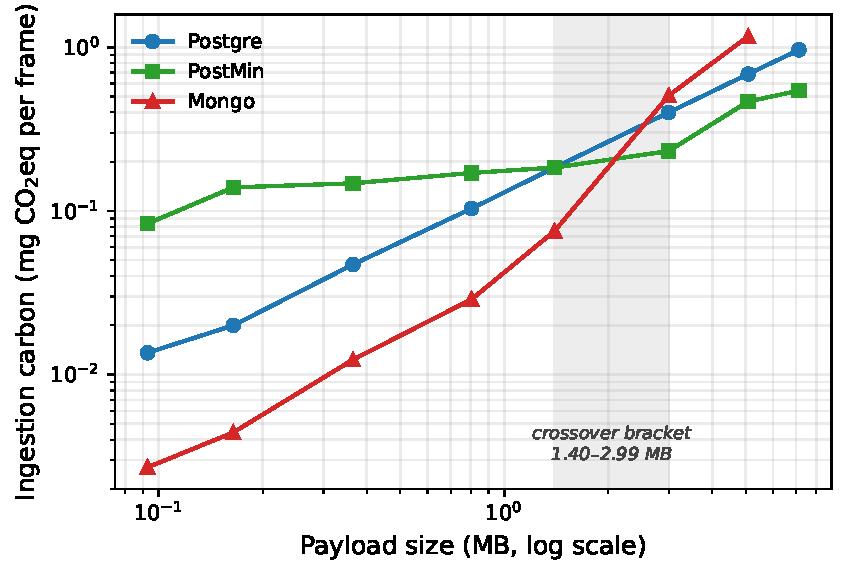
\includegraphics[width=\linewidth]{crossover_collage.pdf}
\caption{Ingestion carbon against payload size across the full collage range, on logarithmic axes. Points are measurements; lines join adjacent points and imply no functional form. MongoDB's per-frame cost rises by more than two orders of magnitude and accelerates beyond roughly one megabyte, as its cache fills and eviction begins to stall writes, which is why no single straight line describes the relationship. Shading marks the bracket between adjacent measurements in which the lowest-carbon architecture changes from MongoDB to the hybrid. MongoDB is absent at 6K because the cell is infeasible rather than merely costly (Section~\ref{subsec:bson}).}\label{fig:crossover_collage}
\end{figure}

\begin{figure}[htbp]
\centering
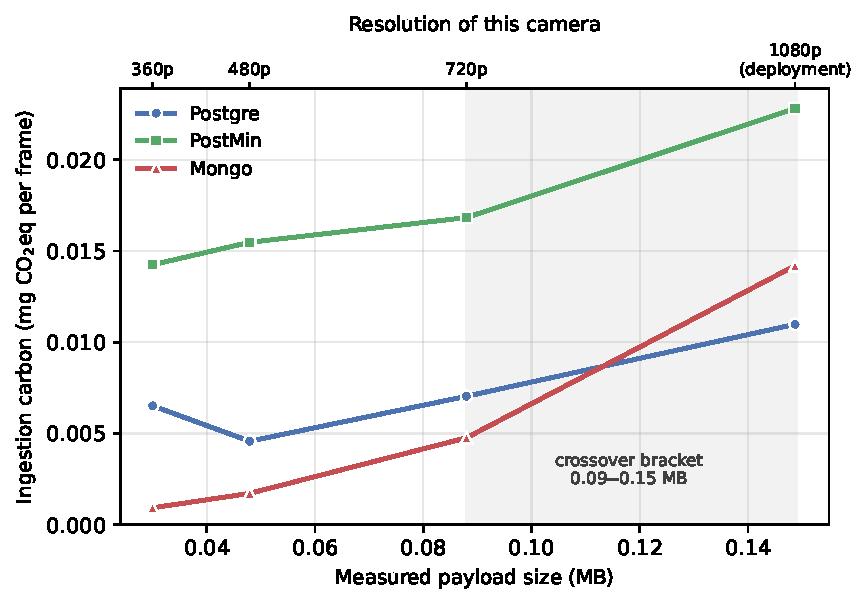
\includegraphics[width=\linewidth]{crossover_realcase.pdf}
\caption{The same measurement for the real-case corpus, over the payload range the deployment actually produces. The upper axis shows where this camera's resolutions fall on the payload axis; the relation between the two is specific to this camera, since another sensor at the same nominal resolutions would place the ticks elsewhere. The crossover bracket lies between $0.09$ and $0.15$~MB, an order of magnitude below the collage bracket of Figure~\ref{fig:crossover_collage}, and the deployment operates at its upper edge. Both the payload and the host contribute to where this boundary falls: changing the payload construction on one machine introduces the transition an order of magnitude earlier (Section~\ref{subsec:sizevsres}), and changing the host moves it by one resolution step (Section~\ref{subsec:twohosts}). The position is therefore specific to an installation and is something to be measured there.}\label{fig:applied}
\end{figure}

\begin{figure}[htbp]
\centering
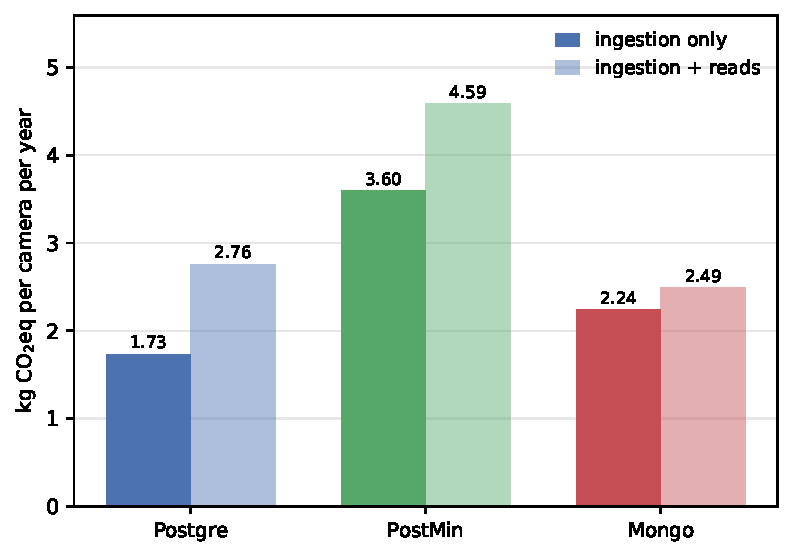
\includegraphics[width=\linewidth]{applied_annual.pdf}
\caption{Annual carbon for one camera of the deployment capturing continuously at 5~frames per second, counting ingestion alone and ingestion together with retrieval and latest-frame reads. The selection inverts between the two: a deployment that stores continuously and reads rarely, as this one does, is governed by the left-hand bars and selects PostgreSQL, whereas weighting reads equally would select MongoDB. This is why operating regime forms an axis of Table~\ref{tab:decision} alongside payload size.}\label{fig:applied2}
\end{figure}

\begin{table}[htbp]
\caption{The framework applied to one camera of the deployment as a scenario projection: 1080p, 5~frames per second, operating continuously, with a measured payload of $0.149$~MB. Carbon is per camera per year; storage is the volume retained at a 90-day retention period. ``Write'' counts ingestion only, which is the regime of a deployment that stores continuously and reads rarely; ``total'' additionally counts bulk retrieval and latest-frame reads.}\label{tab:applied}
\small
\begin{tabular}{@{}lrrrr@{}}
\toprule
Architecture & mg/frame & kg/yr (write) & kg/yr (total) & TB at 90 days \\
\midrule
Postgre & \textbf{0.0110} & \textbf{1.73} & 2.76 & 5.96 \\
Mongo   & 0.0142 & 2.24 & \textbf{2.49} & \textbf{5.34} \\
PostMin & 0.0228 & 3.60 & 4.59 & 5.79 \\
\botrule
\end{tabular}
\footnotetext{At a facility Power Usage Effectiveness of 1.5, the selected architecture totals $2.60$~kg~CO\textsubscript{2}eq per camera per year, or $260$~kg for a hundred-camera site against $540$~kg for the costliest alternative.}
\end{table}

Three observations follow, and the first is the one that matters most for the framework's credibility.

\textbf{The framework does not return the same answer everywhere.} For this deployment it selects inline PostgreSQL, not MongoDB, even though 1080p would sit in MongoDB's band were the bands read as resolutions calibrated on worst-case payloads. The reason is the one Table~\ref{tab:decision} is now stated to capture: the rule keys on measured payload size, and this camera's output is light enough to fall above the ingestion crossover. The measured crossover bracket for this corpus lies between $0.131$ and $0.149$~MB (Section~\ref{subsec:sizevsres}), and this camera's payload of $0.149$~MB sits at its upper edge, on PostgreSQL's side. The annual figures confirm it, at $1.73$ against $2.24$~kg per camera per year. A camera whose output is lighter than the high-entropy worst case falls on the far side of a boundary that a resolution-only rule would have missed entirely.

\textbf{Workload emphasis changes the answer.} Ingestion alone selects PostgreSQL; counting retrieval and latest-frame reads equally would select MongoDB ($2.49$ against $2.76$~kg), and minimising retained volume would also select MongoDB ($5.34$~TB at 90 days). A deployment that stores continuously and reads rarely, as this one does, is squarely in the first regime, which is why the write column governs the choice. The three columns of Table~\ref{tab:applied} are the operating regimes of Table~\ref{tab:decision} made concrete for one site.

\textbf{The saving is modest per camera and material at scale.} Choosing PostgreSQL over the costliest alternative saves $1.86$~kg~CO\textsubscript{2}eq per camera per year, a $52\%$ reduction in the ingestion footprint of the image tier. One camera is negligible; a hundred-camera site saves $280$~kg annually at a Power Usage Effectiveness of $1.5$, for a decision taken once at design time and costing nothing thereafter.

One boundary should be stated plainly. The installation currently retains video rather than individual frames, so these figures project the footprint of an image-based tier for that deployment; they are not a measured saving against its present configuration, and the two storage models are not directly comparable. What the exercise demonstrates is that the framework, given one measured payload size and one capture regime, yields a specific architecture and a specific annual figure for a real installation, which is the use for which it is intended.

\subsection{Alignment with Sustainable Development Goals}\label{subsec:sdg}
Carbon-aware storage selection contributes to several of the United Nations Sustainable Development Goals (SDGs), the 2030 agenda of seventeen global targets for sustainability~\citep{un_sdg}: SDG~7 (affordable and clean energy) and SDG~13 (climate action) through direct reductions in operational and embodied emissions; SDG~9 (industry, innovation, and infrastructure) and SDG~11 (sustainable cities and communities) by informing greener building-monitoring infrastructure; and SDG~12 (responsible consumption and production) by curbing the over-provisioning of storage through amplification-aware design.

%%=====================================================================%%
\section{Discussion}\label{sec:discussion}
%%=====================================================================%%

\subsection{Why the crossover occurs}
Section~\ref{subsec:model} sets out the mechanism; three engine-specific details fill it in. MongoDB writes the entire BSON document, image included, through its on-disk index pages and holds it \emph{uncompressed} in working memory~\citep{wiredtiger_btree_architecture}; as payloads grow, Snappy~\citep{google_snappy} finds little to remove in high-entropy JPEG, storage amplification climbs to $3.00\times$, and at the largest sizes the cache fills, forcing eviction to disk and stalling the writes in progress~\citep{percona_wiredtiger_eviction}. PostgreSQL's TOAST~\citep{postgresql_toast_docs} relocates images out-of-line, keeping the main index compact and the write path roughly independent of resolution ($1.04\times$ amplification), which is what makes its carbon stable and middle-of-the-road. In the hybrid, PostgreSQL records only metadata, so its write-ahead log (WAL, the change journal a database writes before applying updates, used for crash recovery) and indexes grow with the metadata rather than the image, while MinIO streams the object: the most energy-efficient path once payloads are large, at the cost of a fixed HTTP round-trip that makes it the worst choice for small ones.

\subsection{Implications for green building monitoring}
There is no single ``green database,'' and the answer depends on the operation profile as much as on the payload. Under the equal-weight profile, light camera streams are greenest on MongoDB and heavy inspection or surveillance streams on PostgreSQL+MinIO; under an ingestion-only profile, which is what a continuously capturing installation runs, the first boundary moves by an order of magnitude and inline PostgreSQL takes much of the light-payload band as well (Section~\ref{subsec:applied}). Inline PostgreSQL is in any case the safe default when payloads are mixed or unmeasured, or when operational simplicity (a single transactional boundary, simpler backup and recovery) is valued. The 16~MiB bucket ceiling further removes MongoDB from consideration for $\geq$6K media regardless of carbon, under the bucketing configuration a practitioner obtains by default. These map directly to the infrastructure decisions in Table~\ref{tab:decision}.

\subsection{Operational trade-offs}
The hybrid introduces two services with independent failure modes and a two-step write (a database insert plus a MinIO upload) that is not \emph{atomic}---the two steps can succeed or fail independently, so a crash in between can leave an image without its metadata or vice versa---and therefore requires clean-up logic such as periodically deleting orphaned objects. Inline PostgreSQL keeps everything within a single all-or-nothing transaction. These operational costs must be weighed against the hybrid's carbon and storage advantages at high resolution. Because the underlying mechanism---inline large-object handling versus externalised object transport---is generic, the qualitative crossover is expected to transfer to other relational engines with large-object columns, though exact crossover points depend on each engine's page layout and logging. For the same reason we pair the object store with PostgreSQL only: once the payload is externalised, the metadata engine contributes a small, payload-independent overhead, so a MongoDB+MinIO hybrid would closely track PostgreSQL+MinIO. We therefore keep the comparison on the decisive inline-versus-externalised axis rather than adding a fourth, largely redundant arm.

\subsection{Positioning against prior work}
It is worth stating precisely what changes relative to the studies in Table~\ref{tab:relwork}, because the contribution is not a further benchmark but a reversal of one of their conclusions and a reframing of the decision they inform.

Existing time-series benchmarks agree on an engine ordering that we find to be conditional. TSBS~\citep{tsbs} and the CrateDB benchmark~\citep{cratedb_ts_benchmark} rank systems on small scalar rows, and \citet{diva_timescaledb_mongodb_eval} report MongoDB ingesting faster than TimescaleDB on numeric sensor data. Our measurements agree with that direction at small payloads, MongoDB ingesting over $6\times$ faster than inline PostgreSQL at 360p, and then show it does not survive its own premise. The comparison is qualitative rather than a replication: those studies use different data, hardware, and metrics, and what we compare is the direction of the ordering. The ordering inverts between 1440p and 4K, and MongoDB becomes not merely slower but \emph{infeasible} at 6K. What appears in the scalar literature as a property of the engines is in fact a property of the payload regime those benchmarks happen to occupy. This matters beyond our setting: a practitioner selecting a store for image workloads on the strength of scalar benchmarks will select the architecture that is worst at scale, and the published evidence gives no warning, because no scalar benchmark reaches the payload sizes at which the internal layout of the storage engine begins to dominate.

The carbon-accounting literature supplies methods rather than answers at this granularity. \citet{lannelongue_green_algorithms} formalise footprint estimation for computation, \citet{gsf_sci} standardise reporting per unit of useful work, and \citet{gupta_chasing_carbon} and \citet{tannu_ssd_embodied} establish embodied carbon as a first-class concern. All operate above the level of an individual storage operation: they can attribute a footprint to a workload once its energy is known, but not tell an operator which of three architectures will consume that energy. We measure at the granularity the decision actually requires, that is per architecture, per operation, and per resolution, and this is what exposes the crossover. A single aggregate figure per architecture, of the kind these methods would ordinarily produce, would have averaged the crossover away entirely and yielded a spurious universal winner.

Relative to our own earlier conference work [hidden for double-blind review], two things change. Per-resolution carbon is measured directly rather than apportioned from one coarse measurement using a constant power model, which removes an assumption that is now testable and, as Section~\ref{subsec:realframes} shows, would have been misleading in a specific way. And the result is no longer a benchmark table but a decision instrument: the rule is stated in terms of measured payload size, with a procedure for locating the boundaries on other hardware, rather than as a recommendation tied to ours.

The advance we claim is therefore threefold: an inversion, in a payload regime the benchmarks reviewed here do not reach, of the engine ordering they report; an infeasibility result that no hardware removes under the bucketing configuration a practitioner obtains by default; and a transferable calibration procedure in place of a fixed recommendation. The claim we do \emph{not} make is that the specific crossover payloads generalise. They are measurements on one host and one corpus, and Section~\ref{subsec:realframes} shows that even the margins at those resolutions depend on how realistic the payload corpus is.

\subsection{Threats to validity}
The second host's MongoDB measurements are incomplete above 1440p: the 4K cell was terminated by the kernel and 5K and 6K were not reached (Section~\ref{subsec:memory}). Those points lie beyond the payload at which the hybrid has already overtaken MongoDB there, so the omission does not affect the comparison, but it does mean the smaller host's crossover is bracketed on one side only. Run-to-run variability on that host is also markedly higher, up to $28\%$ against under $6\%$ on the larger machine, which is why we report the change in margin rather than a crossover position for it. The measurements cover the data tier only. Where a real-case deployment is used (Section~\ref{subsec:realframes}), it supplies the stored images and the capture regime; its recognition pipeline is neither measured nor modelled, so the figures reported here are not a whole-system footprint for such an installation. Results are otherwise from a single host and container topology; distributed deployments may differ, though the relative comparison holds because all engines ran under identical conditions. Per-resolution emissions are now directly measured (removing the estimation assumption of earlier work [hidden for double-blind review]), but energy accuracy depends on the Intel RAPL counters; on computers where RAPL is unavailable, CodeCarbon falls back to Thermal Design Power (TDP) estimates---nameplate power ratings rather than live measurement. Each cell's carbon is a single integrated CodeCarbon measurement normalised to one run rather than a five-run mean; the low run-to-run variability of the underlying insertion and retrieval timings bounds its uncertainty, and independent repeated energy runs would tighten the per-cell estimate---a straightforward extension. We benchmark a single client issuing requests sequentially, and fix the batch size at~50. Both are deliberate baseline choices: concurrency changes how energy is attributed and introduces contention noise, while larger batches mainly reduce per-round-trip overhead for the inline engines and not the one-object-per-PUT cost of the hybrid. Because the crossover is driven by payload size, a structural property of each design, we expect neither to move the ordering, but multi-client and batch-size sweeps are left as future work rather than claimed. Payloads in the controlled benchmark are deterministic collages built from a single real photograph~\citep{pexels_durdle_door} rather than a diverse image corpus, which is why it is paired with the real-case corpus of Section~\ref{subsec:realframes}: 2{,}845--2{,}988 independently captured frames per camera, on which the ordering is the same and the margins are those of ordinary camera output. Because each stored record is an independent image, its storage, write amplification, and energy cost depend on the payload's size and \emph{entropy} (its compressibility) rather than on its subject matter or on any temporal relationship between frames, so a still image is a representative payload and video would matter only for inter-frame codecs we do not study. Scene diversity nonetheless remains a limitation: a broader corpus would refine the absolute figures, though quality-90 photographic content is already close to a worst case for the inline engines and is not expected to move the inline-versus-externalised ordering. Finally, the embodied-carbon and fleet figures are first-order estimates using representative published factors and stated assumptions, intended to convey magnitude rather than site-specific precision.

%%=====================================================================%%
\section{Conclusion}\label{sec:conclusion}
%%=====================================================================%%

This paper measured the carbon footprint of three storage architectures---document-oriented MongoDB, relational PostgreSQL-BYTEA, and hybrid PostgreSQL+MinIO---for image-based time-series workloads from 360p to 6K, using CodeCarbon with RAPL hardware energy measurement, with carbon measured directly for every architecture, resolution, and operation and a common retrieval workload across all three engines. The key finding is a payload-dependent emission crossover with no universal winner. Under a profile counting one insertion, one bulk retrieval, and one latest-frame read equally, MongoDB is greenest at small payloads, up to 1440p under this workload, the hybrid is greenest from 4K (roughly halving inline-storage carbon and lowest cumulatively, by $\approx$25\%), and inline PostgreSQL is the pivot---while MongoDB is infeasible at 6K on any hardware under the default time-series bucketing, because that bucketing breaches the 16~MiB BSON limit, and proved unrunnable from 4K upward on a memory-constrained host where both other architectures completed the full range. We translated the measurements into a carbon-aware decision framework and supported it with Software Carbon Intensity, multi-region grid sensitivity, embodied-carbon implications of storage amplification, and a fleet-scale projection.

The controlled benchmark is reinforced throughout by a real-case deployment: a corpus of real camera frames, captured from an operational installation on two cameras and measured on a second computer, over which the ordering is the same and the margins are those of ordinary camera output. Payload and environment vary jointly between that experiment and the controlled sweep rather than being isolated, so the ordering is established as consistent across the tested combinations rather than as independent of either. A controlled comparison further shows that the margin, though not the ordering, depends on whether stored rows are distinct, which is a caution for any benchmark of this kind. Future work will extend the study to distributed and multi-client deployments, broaden the real-case corpus above 1080p and across more scenes, broaden the embodied-carbon and PUE accounting with site-specific factors, and validate the decision rule on held-out monitoring workloads. A public artifact---benchmark code, Docker configurations, and raw results---accompanies the paper to support reproduction.

\backmatter

\section*{Statements and Declarations}

\textbf{Funding.} This research did not receive funding.

\textbf{Competing interests.} The authors declare no competing interests.

\textbf{Use of AI-assisted technologies.} Generative AI assistants (Google Gemini, Anthropic Claude via Claude Code, and OpenAI Codex) were used solely for language editing, that is improving the grammar, clarity, and phrasing of text written by the authors. No AI tool was used to generate, analyse, or interpret the experimental data, to produce the figures or tables, or to draw the scientific conclusions reported here. The authors reviewed and edited all such output and take full responsibility for the entire content of this manuscript. AI is not credited as an author, in accordance with the journal's editorial policy.

\textbf{Data and code availability.} A reproducibility artifact accompanies this submission and will be deposited in a public repository with a persistent identifier on acceptance. It contains the benchmark harness, the Docker configurations, the raw per-run measurement CSVs for all six measurement sets reported here (both hosts and all three cameras), the figure-generation scripts, and the manuscript source, so that every table and figure can be rebuilt without re-running the benchmark. The collage source image is redistributable under its original licence. The corpus of real camera frames used in Section~\ref{subsec:realframes} is released in full, as three archives of $2{,}845$, $2{,}988$, and $2{,}891$ frames, one per camera, alongside the recording tool that produced them; the frames are separated from the main archive only so that the code and measurements can be retrieved without them. Each measurement file records the country in which it was taken, since the grid-intensity factor depends on it, but not a finer location.

\textbf{Ethics.} The deployment described in Section~\ref{subsec:realframes} performs face recognition in normal operation, so we state precisely what was done. No recognition function was invoked and no enrolled identity, template, or record was accessed; the cameras were read directly, and the study used only the resulting image files as binary payloads. Recording was carried out by an author in a space with no other person present, and no biometric template was computed or stored at any point. Every saved frame was then passed through a face detector (YuNet, confidence threshold $0.35$) and none produced a detection. We report that as what it is: evidence that the released corpus contains \emph{no detectable faces}, not a proof that it contains no personal data, since a detector sweep cannot establish the latter. The frames are retained only as the study artifact and were not used for identification, recognition, tracking, or any purpose connected with the deployment's normal operation. Institutional guidance was that work of this kind, involving no participants and no processing of biometric data, does not require ethics review; we state the basis rather than assert an approval that was not sought. The images serve only as representative binary payloads for storage measurement, and no identification, recognition, or tracking was performed on them.

\begin{appendices}

\section{Schemas and queries}\label{app:schemas}
This appendix gives, for each architecture, the schema and the three data operations used by the benchmark harness, exactly as issued (columns abbreviated for space). In PostgreSQL (Listing~\ref{lst:pg}) the image is held inline in a \texttt{BYTEA} column of a TimescaleDB hypertable, where TOAST relocates it out-of-line automatically: insertion is a batched parameterised \texttt{INSERT} (50 rows per round-trip), bulk retrieval is a single time-range \texttt{SELECT} streamed through a server-side cursor, and the latest-frame read is an indexed \texttt{ORDER BY ts DESC LIMIT 1}. In MongoDB (Listing~\ref{lst:mongo}) each frame is one document in a native time-series collection with the image inline as \texttt{BinData}; the equivalent operations are an \texttt{insertMany}, a time-range \texttt{find} projected to the payload, and a \texttt{find}/\texttt{sort}/\texttt{limit} for the latest frame. The hybrid (PostMin, Listing~\ref{lst:pm}) shares the relational schema but replaces \texttt{payload\_data BYTEA} with a \texttt{minio\_object\_key TEXT} reference: on insertion the image is uploaded to MinIO with \texttt{put\_object} and only the key is written to PostgreSQL, and each read first fetches the key from PostgreSQL and then streams the object from MinIO with \texttt{get\_object}.

\begin{lstlisting}[language=PgSQL,caption={PostgreSQL-BYTEA (Postgre): TimescaleDB schema and the three data operations (image stored inline as \texttt{BYTEA}).},label={lst:pg}]
-- Schema: hypertable with the image inline as BYTEA (TOAST stores it out-of-line)
CREATE TABLE sensor_media (
  sample_id BIGSERIAL NOT NULL, device_id BIGINT NOT NULL, ts TIMESTAMPTZ NOT NULL,
  payload_data BYTEA NOT NULL, payload_size_bytes INTEGER NOT NULL,
  width INTEGER, height INTEGER, mime_type TEXT NOT NULL,
  PRIMARY KEY (ts, sample_id));
SELECT create_hypertable('sensor_media', by_range('ts'));
CREATE INDEX idx_device_ts_desc ON sensor_media (device_id, ts DESC);

-- Insert: batched, 50 rows per round-trip
INSERT INTO sensor_media (device_id, ts, payload_data, payload_size_bytes, ...)
VALUES (%s, %s, %s, %s, ...);

-- Bulk retrieval: every frame in a time range
SELECT ts, payload_data FROM sensor_media
WHERE device_id = %s AND ts >= %s AND ts <= %s ORDER BY ts;

-- Latest-frame read
SELECT ts, payload_data FROM sensor_media
WHERE device_id = %s ORDER BY ts DESC LIMIT 1;
\end{lstlisting}

\begin{lstlisting}[language=MongoJS,caption={MongoDB (Mongo): native time-series collection schema and the same operations (image stored inline as \texttt{BinData}).},label={lst:mongo}]
// Schema: native time-series collection, image inline as BinData
db.createCollection("sensor_media", {
  timeseries: { timeField: "ts", metaField: "meta", granularity: "seconds" } });
db.sensor_media.createIndex({ "meta.device_id": 1, "ts": -1 });

// Insert: batched, 50 documents per insertMany; each frame is one document
db.sensor_media.insertMany([
  { meta: { device_id: 1, profile: "4k", payload_kind: "image" },
    ts: ISODate("..."), payload_data: BinData(0, "<jpeg bytes>"),
    payload_size_bytes: 3138125, width: 3840, height: 2160, mime_type: "image/jpeg" },
  /* ... */ ]);

// Bulk retrieval: every frame in a time range
db.sensor_media.find(
  { "meta.device_id": 1, ts: { $gte: tMin, $lte: tMax } },
  { ts: 1, payload_data: 1, _id: 0 }).sort({ ts: 1 });

// Latest-frame read
db.sensor_media.find({ "meta.device_id": 1 }).sort({ ts: -1 }).limit(1);
\end{lstlisting}

\begin{lstlisting}[language=PgSQL,caption={PostgreSQL+MinIO (PostMin): the relational schema stores a MinIO object key in place of the image, so each operation pairs a PostgreSQL query with a MinIO HTTP transfer (\texttt{put\_object}/\texttt{get\_object}).},label={lst:pm}]
-- Schema: as Postgre, but the image is replaced by a MinIO object key
CREATE TABLE sensor_media (
  sample_id BIGSERIAL NOT NULL, device_id BIGINT NOT NULL, ts TIMESTAMPTZ NOT NULL,
  minio_object_key TEXT NOT NULL, payload_size_bytes INTEGER NOT NULL,
  width INTEGER, height INTEGER, mime_type TEXT NOT NULL,
  PRIMARY KEY (ts, sample_id));
SELECT create_hypertable('sensor_media', by_range('ts'));
CREATE INDEX idx_device_ts_desc ON sensor_media (device_id, ts DESC);

-- Insert: upload the image to MinIO (HTTP PUT), then store only its key in Postgre
minio.put_object(bucket, key, image_bytes, length, content_type);  -- HTTP PUT
INSERT INTO sensor_media (device_id, ts, minio_object_key, payload_size_bytes, ...)
VALUES (%s, %s, %s, %s, ...);

-- Bulk retrieval: read the keys in a time range, then stream each object from MinIO
SELECT ts, minio_object_key FROM sensor_media
WHERE device_id = %s AND ts >= %s AND ts <= %s ORDER BY ts;
-- for each key:  minio.get_object(bucket, key)                    -- HTTP GET

-- Latest-frame read: newest key from Postgre, then a single object fetch
SELECT ts, minio_object_key FROM sensor_media
WHERE device_id = %s ORDER BY ts DESC LIMIT 1;
-- then:  minio.get_object(bucket, key)                            -- HTTP GET
\end{lstlisting}

\end{appendices}

\bibliography{references}

\end{document}
